\documentclass[]{book}
\usepackage{lmodern}
\usepackage{amssymb,amsmath}
\usepackage{ifxetex,ifluatex}
\usepackage{fixltx2e} % provides \textsubscript
\ifnum 0\ifxetex 1\fi\ifluatex 1\fi=0 % if pdftex
  \usepackage[T1]{fontenc}
  \usepackage[utf8]{inputenc}
\else % if luatex or xelatex
  \ifxetex
    \usepackage{mathspec}
  \else
    \usepackage{fontspec}
  \fi
  \defaultfontfeatures{Ligatures=TeX,Scale=MatchLowercase}
\fi
% use upquote if available, for straight quotes in verbatim environments
\IfFileExists{upquote.sty}{\usepackage{upquote}}{}
% use microtype if available
\IfFileExists{microtype.sty}{%
\usepackage{microtype}
\UseMicrotypeSet[protrusion]{basicmath} % disable protrusion for tt fonts
}{}
\usepackage[margin=1in]{geometry}
\usepackage{hyperref}
\hypersetup{unicode=true,
            pdftitle={Predictive Models: Visualisation, Exploration and Explanation},
            pdfauthor={Przemyslaw Biecek and Tomasz Burzykowski},
            pdfborder={0 0 0},
            breaklinks=true}
\urlstyle{same}  % don't use monospace font for urls
\usepackage{natbib}
\bibliographystyle{apalike}
\usepackage{color}
\usepackage{fancyvrb}
\newcommand{\VerbBar}{|}
\newcommand{\VERB}{\Verb[commandchars=\\\{\}]}
\DefineVerbatimEnvironment{Highlighting}{Verbatim}{commandchars=\\\{\}}
% Add ',fontsize=\small' for more characters per line
\usepackage{framed}
\definecolor{shadecolor}{RGB}{248,248,248}
\newenvironment{Shaded}{\begin{snugshade}}{\end{snugshade}}
\newcommand{\AlertTok}[1]{\textcolor[rgb]{0.94,0.16,0.16}{#1}}
\newcommand{\AnnotationTok}[1]{\textcolor[rgb]{0.56,0.35,0.01}{\textbf{\textit{#1}}}}
\newcommand{\AttributeTok}[1]{\textcolor[rgb]{0.77,0.63,0.00}{#1}}
\newcommand{\BaseNTok}[1]{\textcolor[rgb]{0.00,0.00,0.81}{#1}}
\newcommand{\BuiltInTok}[1]{#1}
\newcommand{\CharTok}[1]{\textcolor[rgb]{0.31,0.60,0.02}{#1}}
\newcommand{\CommentTok}[1]{\textcolor[rgb]{0.56,0.35,0.01}{\textit{#1}}}
\newcommand{\CommentVarTok}[1]{\textcolor[rgb]{0.56,0.35,0.01}{\textbf{\textit{#1}}}}
\newcommand{\ConstantTok}[1]{\textcolor[rgb]{0.00,0.00,0.00}{#1}}
\newcommand{\ControlFlowTok}[1]{\textcolor[rgb]{0.13,0.29,0.53}{\textbf{#1}}}
\newcommand{\DataTypeTok}[1]{\textcolor[rgb]{0.13,0.29,0.53}{#1}}
\newcommand{\DecValTok}[1]{\textcolor[rgb]{0.00,0.00,0.81}{#1}}
\newcommand{\DocumentationTok}[1]{\textcolor[rgb]{0.56,0.35,0.01}{\textbf{\textit{#1}}}}
\newcommand{\ErrorTok}[1]{\textcolor[rgb]{0.64,0.00,0.00}{\textbf{#1}}}
\newcommand{\ExtensionTok}[1]{#1}
\newcommand{\FloatTok}[1]{\textcolor[rgb]{0.00,0.00,0.81}{#1}}
\newcommand{\FunctionTok}[1]{\textcolor[rgb]{0.00,0.00,0.00}{#1}}
\newcommand{\ImportTok}[1]{#1}
\newcommand{\InformationTok}[1]{\textcolor[rgb]{0.56,0.35,0.01}{\textbf{\textit{#1}}}}
\newcommand{\KeywordTok}[1]{\textcolor[rgb]{0.13,0.29,0.53}{\textbf{#1}}}
\newcommand{\NormalTok}[1]{#1}
\newcommand{\OperatorTok}[1]{\textcolor[rgb]{0.81,0.36,0.00}{\textbf{#1}}}
\newcommand{\OtherTok}[1]{\textcolor[rgb]{0.56,0.35,0.01}{#1}}
\newcommand{\PreprocessorTok}[1]{\textcolor[rgb]{0.56,0.35,0.01}{\textit{#1}}}
\newcommand{\RegionMarkerTok}[1]{#1}
\newcommand{\SpecialCharTok}[1]{\textcolor[rgb]{0.00,0.00,0.00}{#1}}
\newcommand{\SpecialStringTok}[1]{\textcolor[rgb]{0.31,0.60,0.02}{#1}}
\newcommand{\StringTok}[1]{\textcolor[rgb]{0.31,0.60,0.02}{#1}}
\newcommand{\VariableTok}[1]{\textcolor[rgb]{0.00,0.00,0.00}{#1}}
\newcommand{\VerbatimStringTok}[1]{\textcolor[rgb]{0.31,0.60,0.02}{#1}}
\newcommand{\WarningTok}[1]{\textcolor[rgb]{0.56,0.35,0.01}{\textbf{\textit{#1}}}}
\usepackage{longtable,booktabs}
\usepackage{graphicx,grffile}
\makeatletter
\def\maxwidth{\ifdim\Gin@nat@width>\linewidth\linewidth\else\Gin@nat@width\fi}
\def\maxheight{\ifdim\Gin@nat@height>\textheight\textheight\else\Gin@nat@height\fi}
\makeatother
% Scale images if necessary, so that they will not overflow the page
% margins by default, and it is still possible to overwrite the defaults
% using explicit options in \includegraphics[width, height, ...]{}
\setkeys{Gin}{width=\maxwidth,height=\maxheight,keepaspectratio}
\IfFileExists{parskip.sty}{%
\usepackage{parskip}
}{% else
\setlength{\parindent}{0pt}
\setlength{\parskip}{6pt plus 2pt minus 1pt}
}
\setlength{\emergencystretch}{3em}  % prevent overfull lines
\providecommand{\tightlist}{%
  \setlength{\itemsep}{0pt}\setlength{\parskip}{0pt}}
\setcounter{secnumdepth}{5}
% Redefines (sub)paragraphs to behave more like sections
\ifx\paragraph\undefined\else
\let\oldparagraph\paragraph
\renewcommand{\paragraph}[1]{\oldparagraph{#1}\mbox{}}
\fi
\ifx\subparagraph\undefined\else
\let\oldsubparagraph\subparagraph
\renewcommand{\subparagraph}[1]{\oldsubparagraph{#1}\mbox{}}
\fi

%%% Use protect on footnotes to avoid problems with footnotes in titles
\let\rmarkdownfootnote\footnote%
\def\footnote{\protect\rmarkdownfootnote}

%%% Change title format to be more compact
\usepackage{titling}

% Create subtitle command for use in maketitle
\newcommand{\subtitle}[1]{
  \posttitle{
    \begin{center}\large#1\end{center}
    }
}

\setlength{\droptitle}{-2em}

  \title{Predictive Models: Visualisation, Exploration and Explanation}
    \pretitle{\vspace{\droptitle}\centering\huge}
  \posttitle{\par}
    \author{Przemyslaw Biecek and Tomasz Burzykowski}
    \preauthor{\centering\large\emph}
  \postauthor{\par}
      \predate{\centering\large\emph}
  \postdate{\par}
    \date{2018-09-14}

\usepackage{booktabs}

\usepackage{amsthm}
\newtheorem{theorem}{Theorem}[chapter]
\newtheorem{lemma}{Lemma}[chapter]
\theoremstyle{definition}
\newtheorem{definition}{Definition}[chapter]
\newtheorem{corollary}{Corollary}[chapter]
\newtheorem{proposition}{Proposition}[chapter]
\theoremstyle{definition}
\newtheorem{example}{Example}[chapter]
\theoremstyle{definition}
\newtheorem{exercise}{Exercise}[chapter]
\theoremstyle{remark}
\newtheorem*{remark}{Remark}
\newtheorem*{solution}{Solution}
\begin{document}
\maketitle

{
\setcounter{tocdepth}{1}
\tableofcontents
}
\hypertarget{introduction}{%
\chapter{Introduction}\label{introduction}}

Machine Learning (ML) models have a wide range of applications in
classification or regression problems. Due to the increasing
computational power of computers and complexity of data sources, ML
models are becoming more and more sophisticated. Models created with the
use of techniques such as boosting or bagging of neural networks are
parametrized by thousands of coefficients. They are obscure; it is hard
to trace the link between input variables and model outcomes - in fact
they are treated as black boxes. They are used because of their
elasticity and high performance, but their deficiency in
interpretability is one of their weakest sides.

In many applications we need to know, understand or prove how the input
variables are used in the model. We need to know the impact of
particular variables on the final model predictions. Thus we need tools
that extract useful information from thousands of model parameters.

Fully trained models

\hypertarget{model-lifecycle}{%
\section{Model Lifecycle}\label{model-lifecycle}}

\begin{figure}
\centering
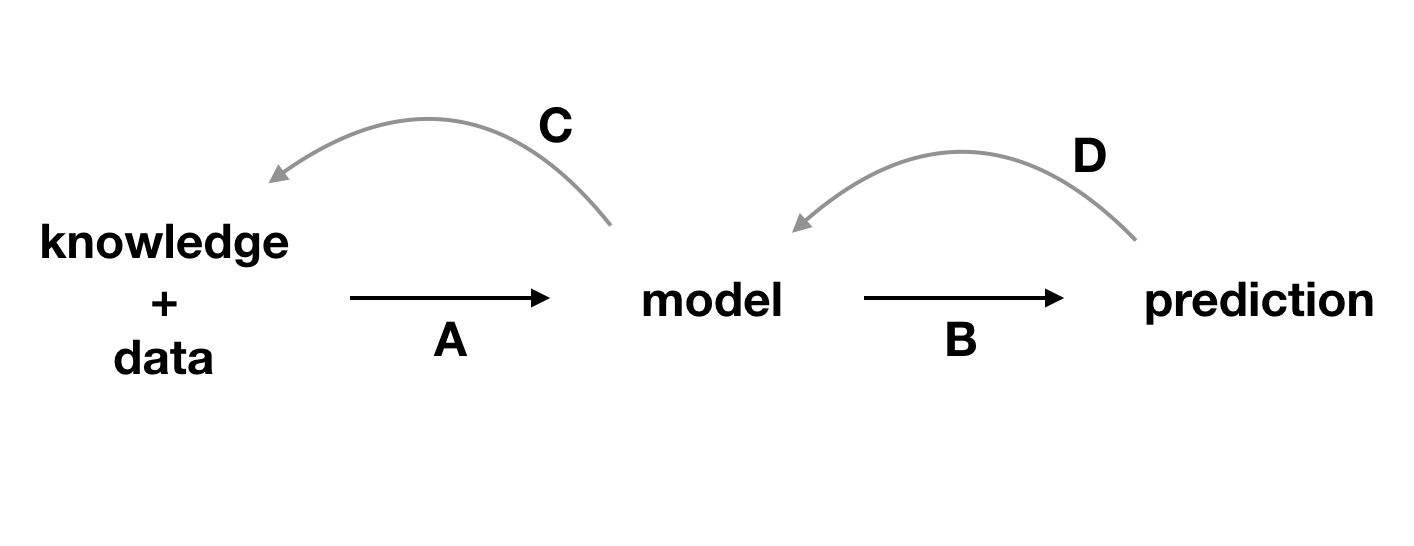
\includegraphics{figure/mp_understanding.png}
\caption{Workflow of a typical machine learning modeling. A) Modeling is
a process in which domain knowledge and data are turned into models. B)
Models are used to generate predictions. C) Understanding of a model
structure may increase our knowledge, and in consequence it may lead to
a better model. DALEX helps here. D) Understanding of drivers behind a
particular model's predictions may help to correct wrong decisions, and
in consequence it leads to a better model. DALEX helps here.}
\end{figure}

Variable importance

Model response as a function of a variable

Model performance / diagnostic / validation

\hypertarget{why-do-we-need-model-explainers}{%
\section{Why do we need model
explainers?}\label{why-do-we-need-model-explainers}}

AutoML

Feature Extraction

Model Improvement

\hypertarget{black-box-models-vs-white-box-models}{%
\section{Black-box models vs White-box
models}\label{black-box-models-vs-white-box-models}}

\citep{R-DALEX}

\hypertarget{model-agnostic-vs-model-specific}{%
\section{Model agnostic vs Model
specific}\label{model-agnostic-vs-model-specific}}

\hypertarget{glossary-notation}{%
\section{Glossary / Notation}\label{glossary-notation}}

feature / variable

Let \(f_{M}(x): \mathcal R^{d} \rightarrow \mathcal R\) denote a
predictive model, i.e.~function that takes \(d\) dimensional vector and
calculate numerical score. In section in which we work with larger
number of models we use subscript \(M\) to index models. But to simplify
notation, this subscript is omitted if profiles for only one model are
considered.

Symbol \(x \in \mathcal R^d\) refers to a point in the feature space. We
use subscript \(x_i\) to refer to a different data points and
superscript \(x^j\) to refer to specific dimensions. Additionally, let
\(x^{-j}\) denote all coordinates except \(j\)-th and let \(x|^j=z\)
denote a data point \(x^*\) with all coordinates equal to \(x\) except
coordinate \(j\) equal to value \(z\). I.e.
\(\forall_{i \neq {j}} x^i = x^{*,i}\) and \(x^j = z\). In other words
\(x|^j=z\) denote a \(x\) with \(j\)th coordinate changed to \(z\).

Now we can define Ceteris Paribus Profile for model \(f\), variable
\(j\) and point \(x\) as

\[
CP^{f, j, x}(z) := f(x|^j = z).
\] I.e. CP profile is a model response obtained for observations created
based on \(x\) with \(j\) coordinated changes and all other coordinates
kept unchanged.

It is convenient to use an alternative name for this plot: What-If
Plots. CP profiles show what would happen if only a single variable is
changed.

Figure 5.1 shows an example of Ceteris Paribus profile. The black dot
stands for prediction for a single observation. Grey line show how the
model response would change if in this single observation coordinate
\texttt{surface} will be changes to selected value. From this profile
one may read that the model response is non monotonic. If
\texttt{construction.year} for this observation would be below 1935 the
model response would be higher, but if construction year were between
1935 and 1995 the model response would be lower.

\hypertarget{thanksto}{%
\section{Thanks to}\label{thanksto}}

We are using the \textbf{bookdown} package \citep{R-bookdown} in this
sample book

Chris Drake and Janusz Holyst

\hypertarget{prediction-level-explanations}{%
\chapter*{Prediction level
explanations}\label{prediction-level-explanations}}
\addcontentsline{toc}{chapter}{Prediction level explanations}

\hypertarget{PredictionExplainers}{%
\chapter{Introduction}\label{PredictionExplainers}}

Prediction level explainers help to understand how the model works for a
single prediction. This is the main difference from the model level
explainers that were focused on the model in general. Prediction level
explainers are always in context of a single observation.

Think about following use-cases

\begin{itemize}
\tightlist
\item
  One wants to attribute effects of variables to a model predictions.
  Think about model for hart attack. Having a final score for a patient
  one wants to understand how much of this score come from smoking or
  age or gender.
\item
  One wants to understand how the model response would change if some
  inputs are changed. Think about model for hart attack. How the model
  response would change if a patient cuts the number of smoked
  cigarettes by half.
\item
  Model is not working correctly for a particular point and one wants to
  understand why predictions for this point are wrong.
\end{itemize}

\hypertarget{variable-atribution-vs-what-if-analysis}{%
\section{Variable atribution vs What-if
analysis}\label{variable-atribution-vs-what-if-analysis}}

There are many different tools that may be used to explore model around
a single data point and in following sections we will describe the most
popular approaches. They can be divided into two classes.

\begin{itemize}
\tightlist
\item
  Analysis of the model curvature. Here we treat the model as a function
  and we are interested in the curvature of this function around the
  point of interest (see Figure \ref{fig:modelResponseCurve}). In
  section \ref{LIME} we present the LIME method that approximates the
  black-box model in a point of interest while in section
  \ref{ceterisParibus} we present Ceteris Paribus profiles that are more
  focused on conditional changes of model response given only one
  coordinate is modified.
\item
  Analysis of the probabilistic behavior of the model. Here we are
  interested in decomposition of the model response to parts that can be
  attributed to particular features.
\end{itemize}

\begin{figure}
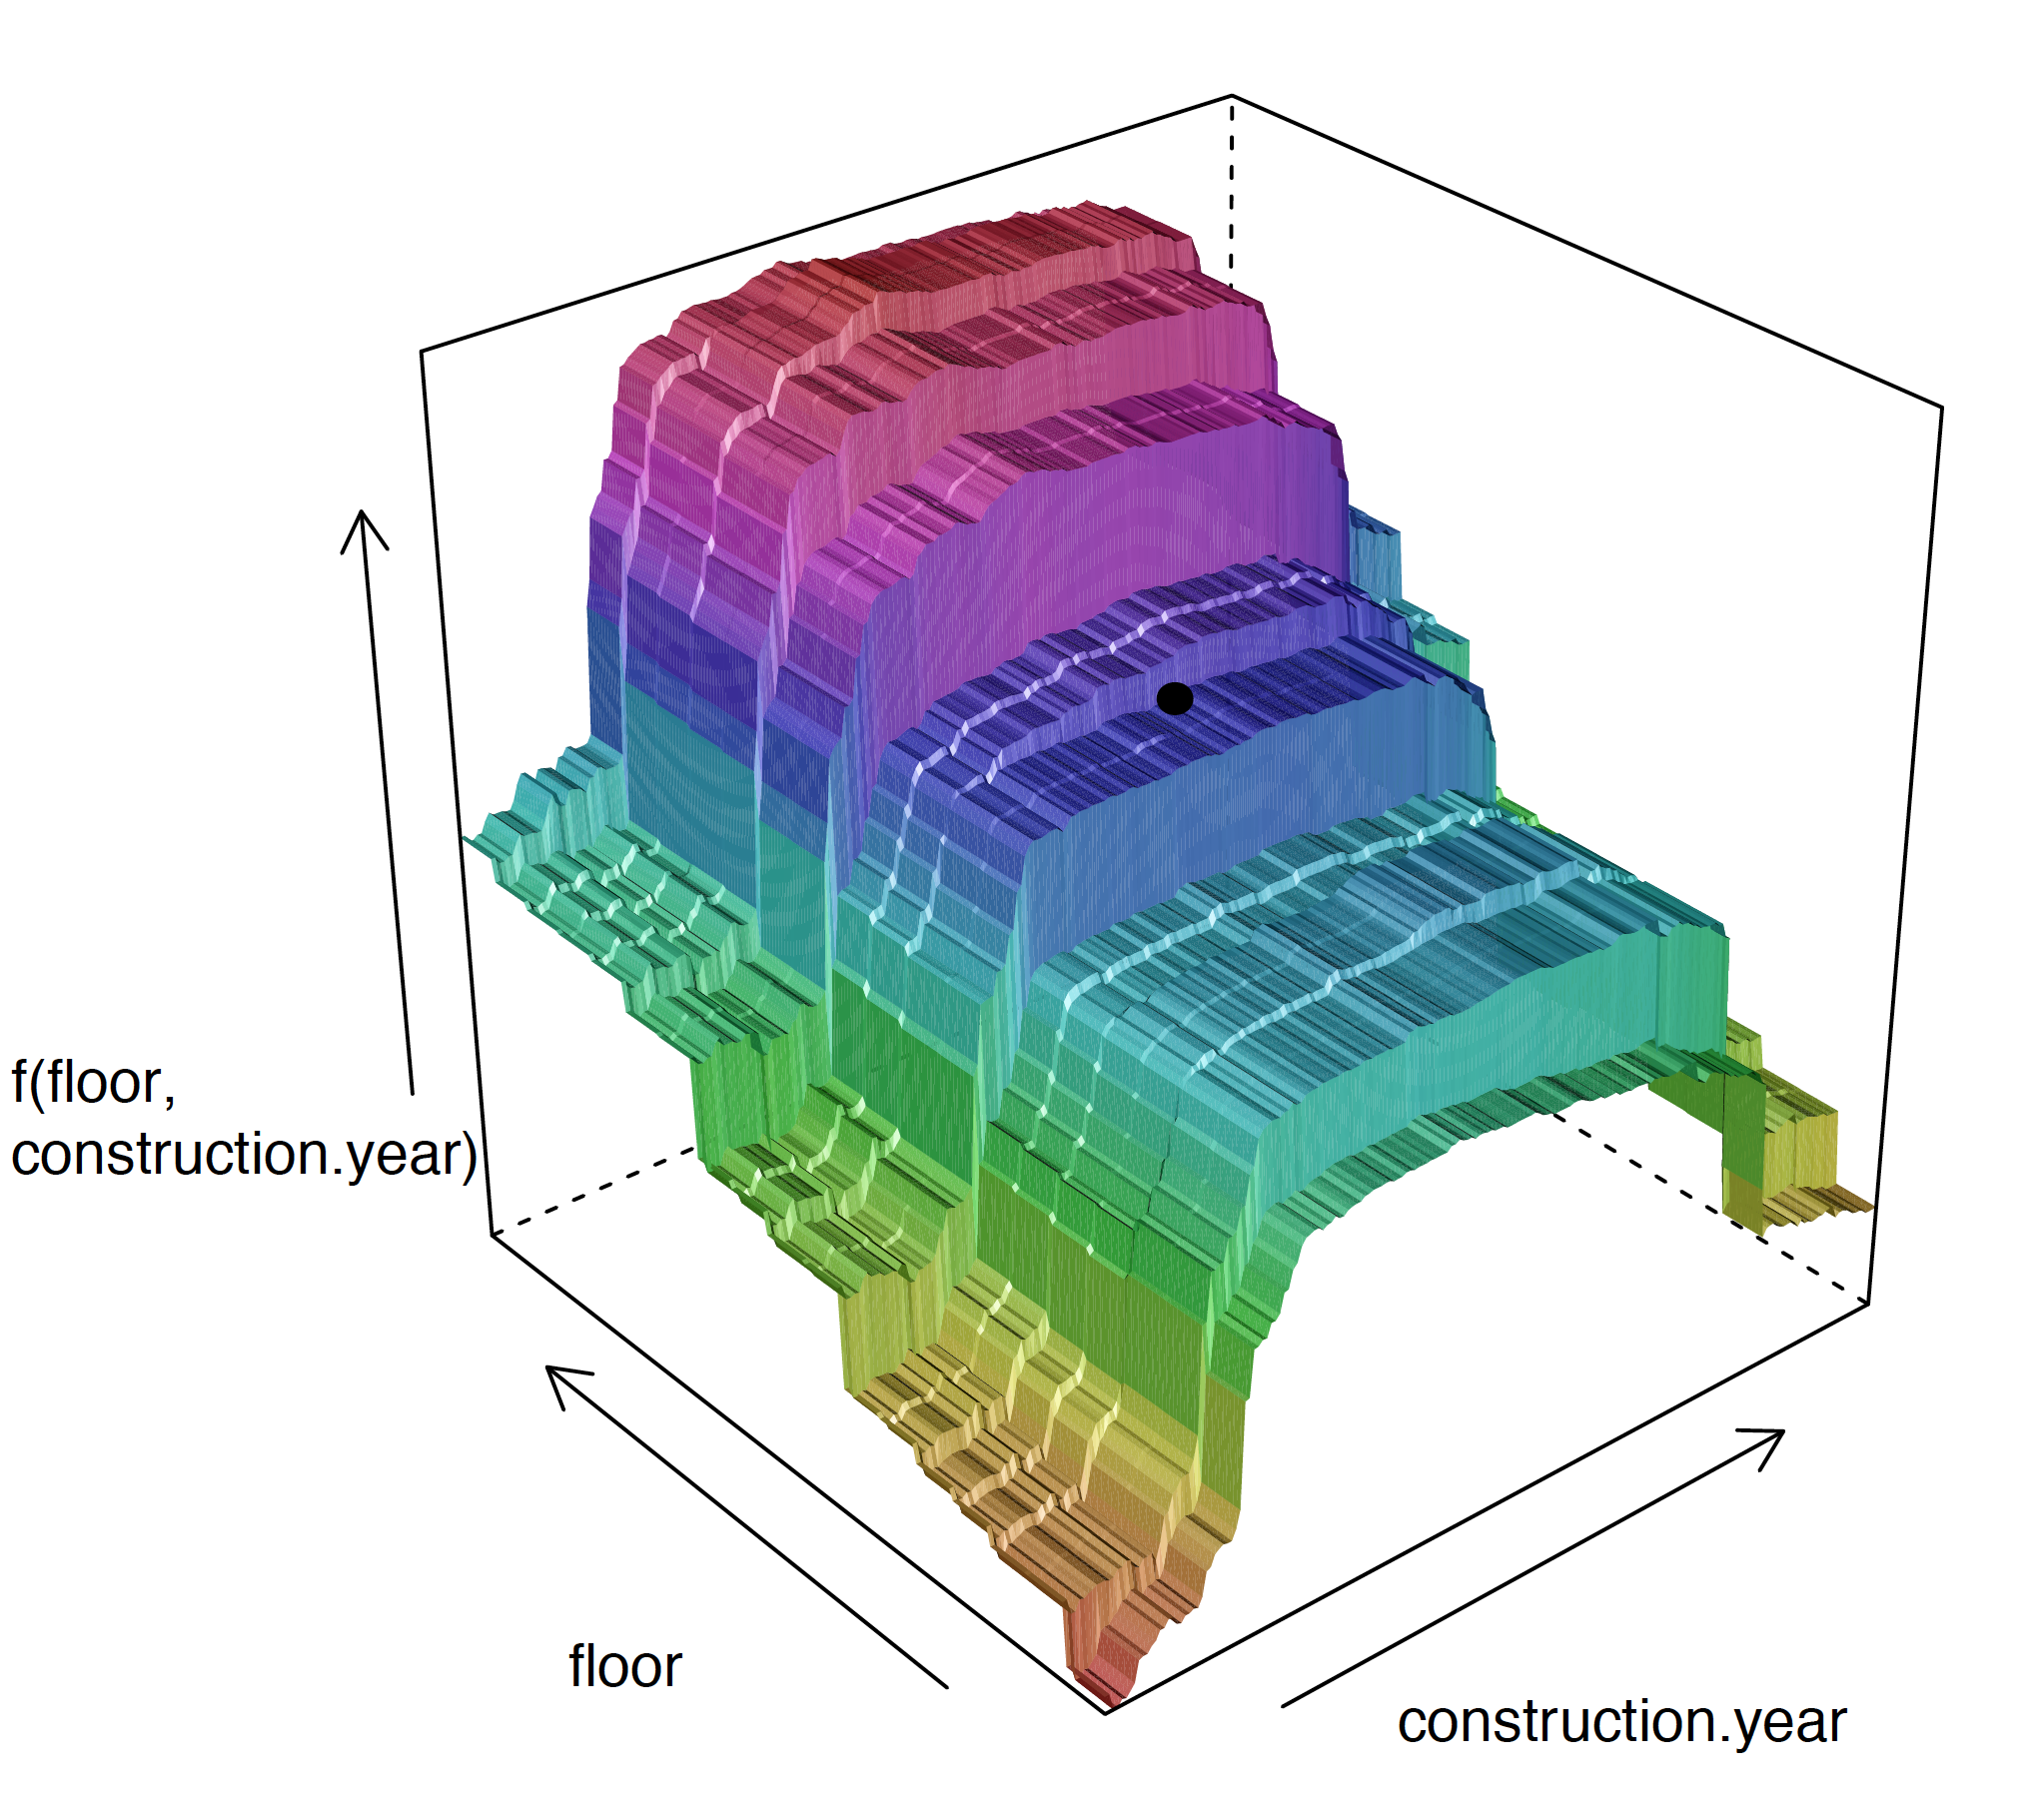
\includegraphics[width=0.7\linewidth]{figure/model_response} \caption{(fig:modelResponseCurve) Model response surface. We are interested in understanding the model behavior in a single point}\label{fig:modelResponseCurve}
\end{figure}

\hypertarget{when-to-use}{%
\section{When to use?}\label{when-to-use}}

There are several use-cases for such explainers. Think about following.

\begin{itemize}
\tightlist
\item
  Model improvement. If model works particular bad for a selected
  observation (the residual is very high) then investigation of model
  responses for miss fitted points may give some hints how to improve
  the model. For individual predictions it is easier to notice that
  selected variable should have different a effect.
\item
  Additional domain specific validation. Understanding which factors are
  important for model predictions helps to be critical about model
  response. If model contributions are against domain knowledge then we
  may be more skeptical and willing to try another model. On the other
  hand, if the model response is aligned with domain knowledge we may
  trust more in these responses. Such trust is important in decisions
  that may lead to serious consequences like predictive models in
  medicine.
\item
  Model selection. Having multiple candidate models one may select the
  final response based on model explanations. Even if one model is
  better in terms of global model performance it may happen that locally
  other model is better fitted. This moves us towards model
  consultations that identify different options and allow human to
  select one of them.
\end{itemize}

\hypertarget{three-single-laws}{%
\section{A bit of philosophy: Three Laws for Prediction Level
Explanations}\label{three-single-laws}}

76 years ago Isaac Asimov devised
\href{https://en.wikipedia.org/wiki/Three_Laws_of_Robotics}{Three Laws
of Robotics}: 1) a robot may not injure a human being, 2) a robot must
obey the orders given it by human beings and 3) A robot must protect its
own existence. These laws impact discussion around
\href{https://en.wikipedia.org/wiki/Ethics_of_artificial_intelligence}{Ethics
of AI}. Today's robots, like cleaning robots, robotic pets or autonomous
cars are far from being conscious enough to be under Asimov's ethics.

Today we are surrounded by complex predictive algorithms used for
decision making. Machine learning models are used in health care,
politics, education, judiciary and many other areas. Black box
predictive models have far larger influence on our lives than physical
robots. Yet, applications of such models are left unregulated despite
many examples of their potential harmfulness. See \emph{Weapons of Math
Destruction} by Cathy O'Neil for an excellent overview of potential
problems.

It's clear that we need to control algorithms that may affect us. Such
control is in our civic rights. Here we propose three requirements that
any predictive model should fulfill.

\begin{itemize}
\tightlist
\item
  \textbf{Prediction's justifications}. For every prediction of a model
  one should be able to understand which variables affect the prediction
  and how strongly. Variable attribution to final prediction.
\item
  \textbf{Prediction's speculations}. For every prediction of a model
  one should be able to understand how the model prediction would change
  if input variables were changed. Hypothesizing about what-if
  scenarios.
\item
  \textbf{Prediction's validations} For every prediction of a model one
  should be able to verify how strong are evidences that confirm this
  particular prediction.
\end{itemize}

There are two ways to comply with these requirements. One is to use only
models that fulfill these conditions by design. White-box models like
linear regression or decision trees. In many cases the price for
transparency is lower performance. The other way is to use approximated
explainers -- techniques that find only approximated answers, but work
for any black box model. Here we present such techniques.

\hypertarget{example-promoted-or-fired}{%
\section{Example: Promoted or Fired?}\label{example-promoted-or-fired}}

In this chapter we will use artificial dataset from Human Resources
department in a call center to present pros and cons for different
techniques of prediction level explainers. At the end of each section
there is a collection of examples that shows how to use described
techniques in R and Python.

The dataset is available in the \texttt{DALEX} package \citep{R-DALEX}.
Each row corresponds to a single employee of a call center. Features
like gender, age, average number of working hours per week, grade from
the last evaluation and level of salary are used as predictive features.

The problem here is to first build a model, that will determine when to
fires and when to promote an employer, so it's a classification problem
with three classes. But having a model we will use prediction level
explainers to better understand how the model works for selected cases.

\begin{Shaded}
\begin{Highlighting}[]
\KeywordTok{library}\NormalTok{(}\StringTok{"DALEX"}\NormalTok{)}
\KeywordTok{head}\NormalTok{(HR)}
\end{Highlighting}
\end{Shaded}

\begin{verbatim}
##   gender      age    hours evaluation salary   status
## 1   male 32.58267 41.88626          3      1    fired
## 2 female 41.21104 36.34339          2      5    fired
## 3   male 37.70516 36.81718          3      0    fired
## 4 female 30.06051 38.96032          3      2    fired
## 5   male 21.10283 62.15464          5      3 promoted
## 6   male 40.11812 69.53973          2      0    fired
\end{verbatim}

In this book we are focused on model exploration rather than model
building, thus for sake ok simplicity we will use two default models
created with random forest \citep{R-randomForest} and generalized linear
model \citep{R-nnet}.

\begin{Shaded}
\begin{Highlighting}[]
\KeywordTok{set.seed}\NormalTok{(}\DecValTok{59}\NormalTok{)}
\KeywordTok{library}\NormalTok{(}\StringTok{"randomForest"}\NormalTok{)}
\NormalTok{model_rf <-}\StringTok{ }\KeywordTok{randomForest}\NormalTok{(status }\OperatorTok{~}\StringTok{ }\NormalTok{gender }\OperatorTok{+}\StringTok{ }\NormalTok{age }\OperatorTok{+}\StringTok{ }\NormalTok{hours }\OperatorTok{+}\StringTok{ }\NormalTok{evaluation }\OperatorTok{+}\StringTok{ }\NormalTok{salary, }\DataTypeTok{data =}\NormalTok{ HR)}

\KeywordTok{library}\NormalTok{(}\StringTok{"nnet"}\NormalTok{)}
\NormalTok{model_glm <-}\StringTok{ }\KeywordTok{multinom}\NormalTok{(status }\OperatorTok{~}\StringTok{ }\NormalTok{gender }\OperatorTok{+}\StringTok{ }\NormalTok{age }\OperatorTok{+}\StringTok{ }\NormalTok{hours }\OperatorTok{+}\StringTok{ }\NormalTok{evaluation }\OperatorTok{+}\StringTok{ }\NormalTok{salary, }\DataTypeTok{data =}\NormalTok{ HR)}
\end{Highlighting}
\end{Shaded}

\begin{verbatim}
## # weights:  21 (12 variable)
## initial  value 8620.810629 
## iter  10 value 7002.127738
## iter  20 value 6239.478146
## iter  20 value 6239.478126
## iter  20 value 6239.478124
## final  value 6239.478124 
## converged
\end{verbatim}

\hypertarget{break-down}{%
\chapter{Break Down}\label{break-down}}

In this section we introduce tools based on variable relaxation
principle. The main goal for these tools is to help understand how model
output may be attributed to input variables or sets of variables.
Attribution is in most cases additive, thus the model response is
decomposed into parts that may be assigned to variables.

Presented explainers are linked with the first law introduced in Section
\ref{three-single-laws}, i.e.~law for prediction's justifications. Note
that there are more tools for variable attribution, some of them will be
presented in next sections.

Think of following use cases:

\begin{itemize}
\tightlist
\item
  Think about a model for hart attack. A patient wants to know which
  factors have highest impact on the final heart risk score.
\item
  Think about a model for apartment prices. An investor wants to know
  how much of the final price may be attributed to the location of an
  apartment.
\item
  Think about a model for credit scoring. A customer wants to know if
  factors like gender, age or number of kids influence model decisions.
\end{itemize}

\hypertarget{introduction-1}{%
\section{Introduction}\label{introduction-1}}

The name \emph{Break Down Plots} comes from the way how Break Down plots
are working. The main goal is to decompose model predictions into parts
that can be additively attributed to particular variables. See an
example in Figure \ref{fig:BDPrice1}.

It is straightforward for linear (and more general: additive) models.
But not that obvious for more complex models. In this section we present
uniform, model agnostic approach to variable attribution.

\begin{figure}

{\centering 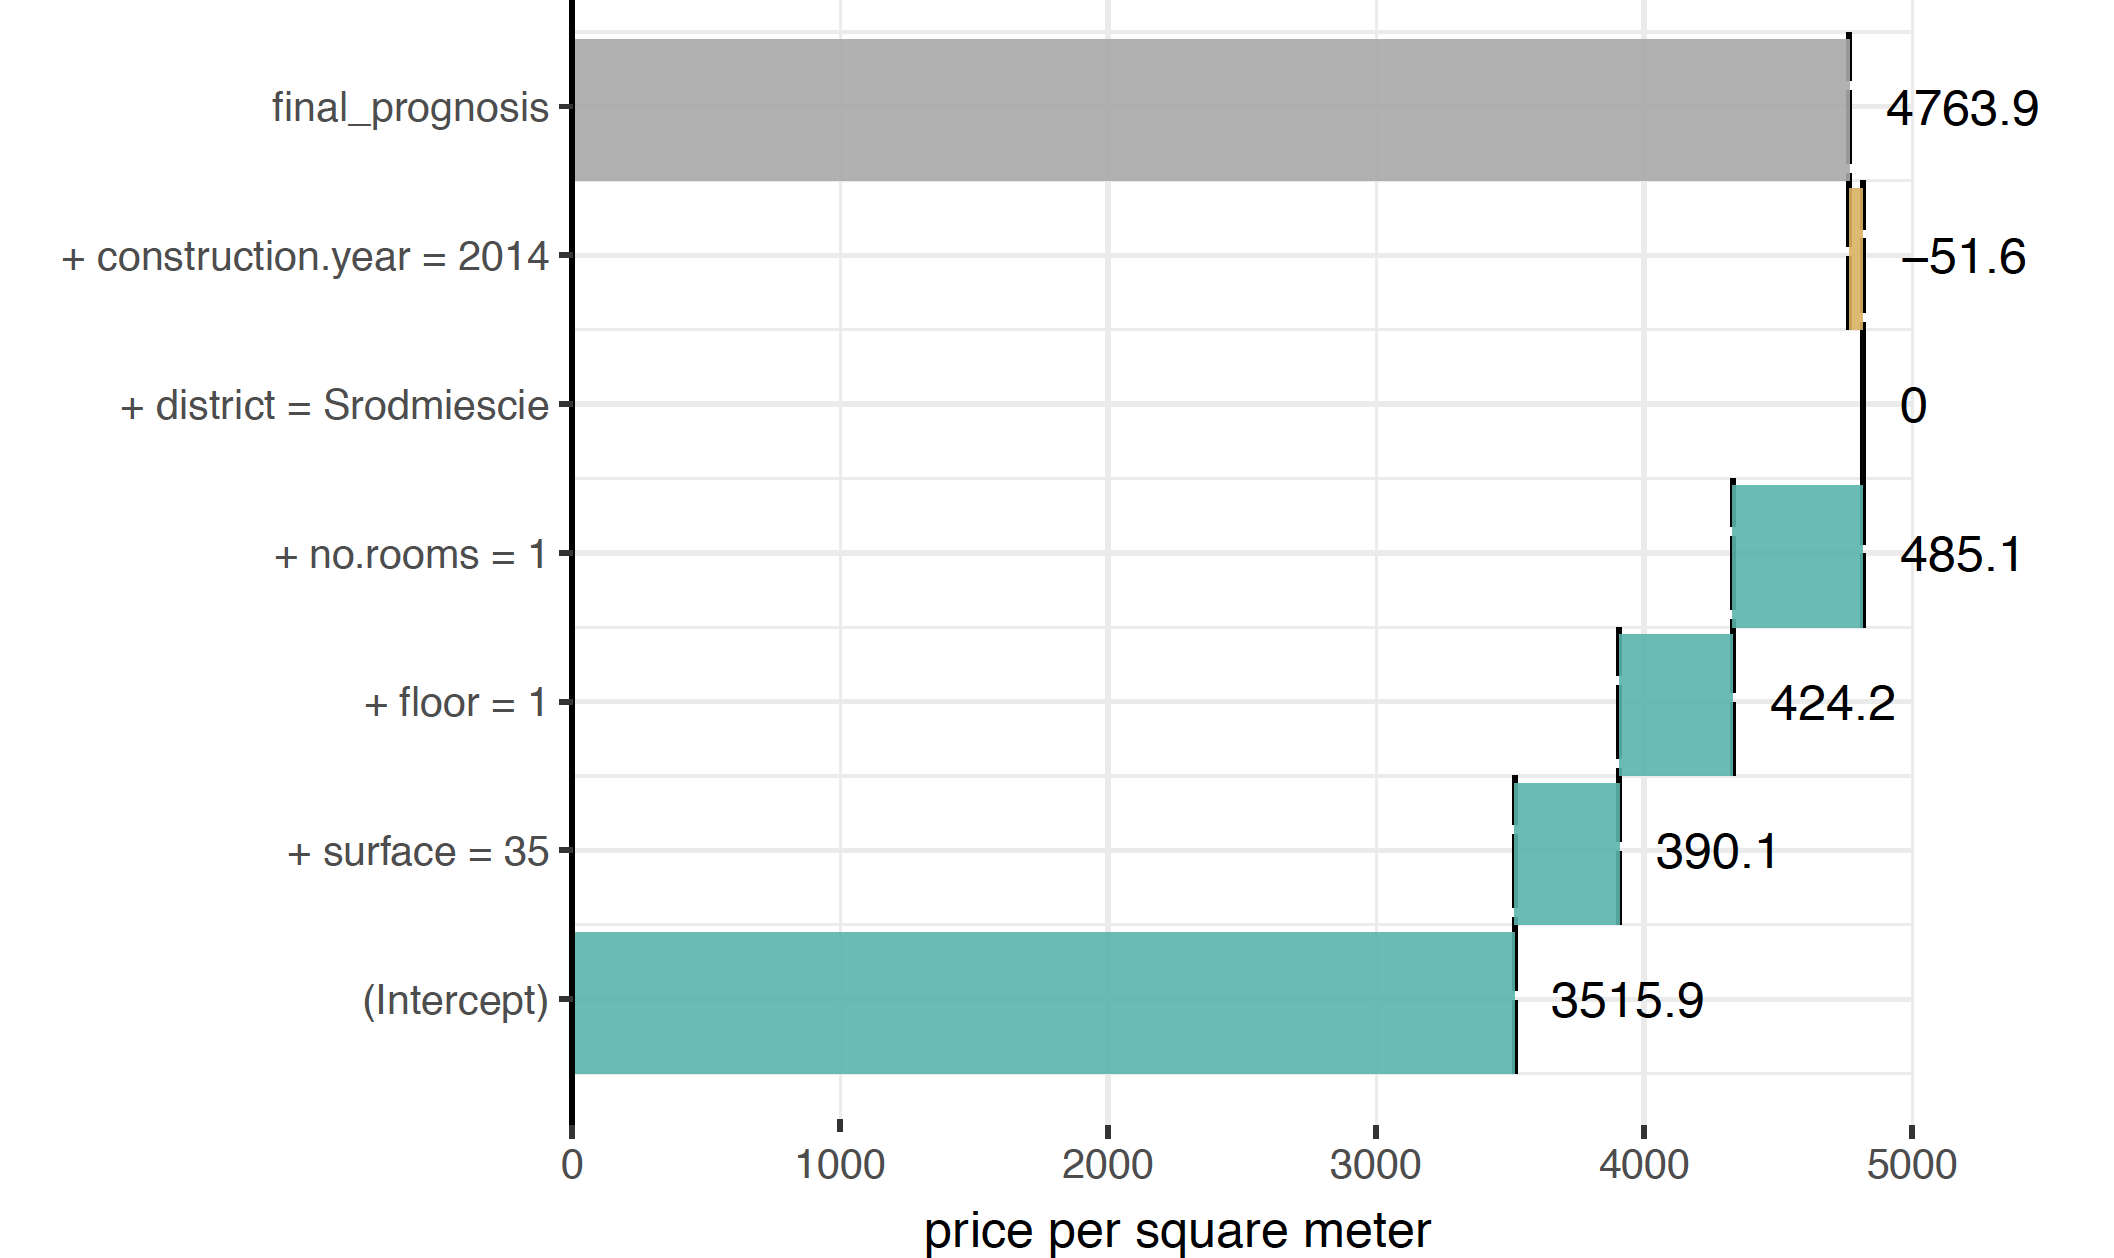
\includegraphics[width=0.7\linewidth]{figure/bd_price_1} 

}

\caption{(fig:BDPrice1) An illustration of Break Down Plots. Model prediction for Random Forest models for a single observation (grey bar, 4763.9) is decomposed into parts that can be attributed to population average (the bottom bar, 3515.9) and effects of particular variables. }\label{fig:BDPrice1}
\end{figure}

Similar to the Shapley method introduced in the Section \ref{shapley},
Break Down Plots show additive decomposition of model output. As we will
show later, the Shapely method may be perceived as an average from all
possible Break Down Paths. In the last subsection we discuss pros and
cons of this approach.

\hypertarget{how-to-read-break-down-plots}{%
\section{How to read Break Down
Plots?}\label{how-to-read-break-down-plots}}

The intuition behind \emph{Break Down} Plots is to show how model
prediction would change if observations in general population will be
made more similar to the observation of interest.

This idea is described in Figure \ref{BDPrice4} and let's trace it step
by step. For a black-box model (here random forest model, but it's
structure is not relevant) we want to decompose prediction for following
point:

\begin{itemize}
\tightlist
\item
  surface: 35
\item
  floor: 1
\item
  no.rooms: 1
\item
  district: Srodmiescie
\item
  construction year: 2014
\end{itemize}

The model prediction is 4763.9. How to attribute following features to
it?

Baseline for this decomposition is the distribution of model predictions
for whole population. In the last row of panel A denoted by
\texttt{all\ data} the violin plot shows distribution of model
prediction for whole population (here calculated on the validation
dataset). Red dot stand for the average, and the average model
prediction, averaged over all points is 3515.9.

Then we check how model prediction would change, if every observation in
the population would have variable \texttt{surface} equal to
\texttt{35}. New distribution for these modified observation is
presented in the second row \texttt{+\ surface\ =\ 35}. Black intervals
between these two rows show how individual prediction change from
original model prediction to the prediction calculated with coordinate
\texttt{surface} set to \texttt{35}. Again, the red dot stands for the
average from model predictions for such modified population. This time
the average is 3906.

In the next step we modify all observations in the population again,
this time we set the \texttt{floor} variable to \texttt{1}. Again, model
prediction will change and black intervals show how individual
prediction change. Also the average from all these modified prediction
will change. This time the new average is 4330.2.

Such steps are repeated for consecutive variables till all variables are
set to the point of interest. In this last step all observations in the
population will have coordinates changed to the observation of interests
and all model predictions are equal 4763.9.

Tracing distributions is not easy, thus instead of distributions we are
focused on averages. Panel B) shows how the average of distribution
changes after each step. The average for whole population was 3515.9.
After setting \texttt{surface} to \texttt{35} the average changed by
\texttt{+390.1}. In the next step, when all observations were changed to
\texttt{floor\ =\ 1} the average changed by \texttt{+424.1}.

Break Down Plots, presented in the panel C) shows only these
differences. Positive values are presented with green bars while
negative differences are marked with yellow bar. They sum up to final
model prediction, which is denoted by a grey bar in this example.

\textbf{NOTE}

If the considered model is additive, then the order in which variables
are added does not matter. If the model is not additive, then different
orders will lead to different effects.

Simplest way to choose an order is to use a greedy procedure in which we
first include variables with largest influence to the average.

Find more details about to this procedure in the next section.

\begin{figure}

{\centering 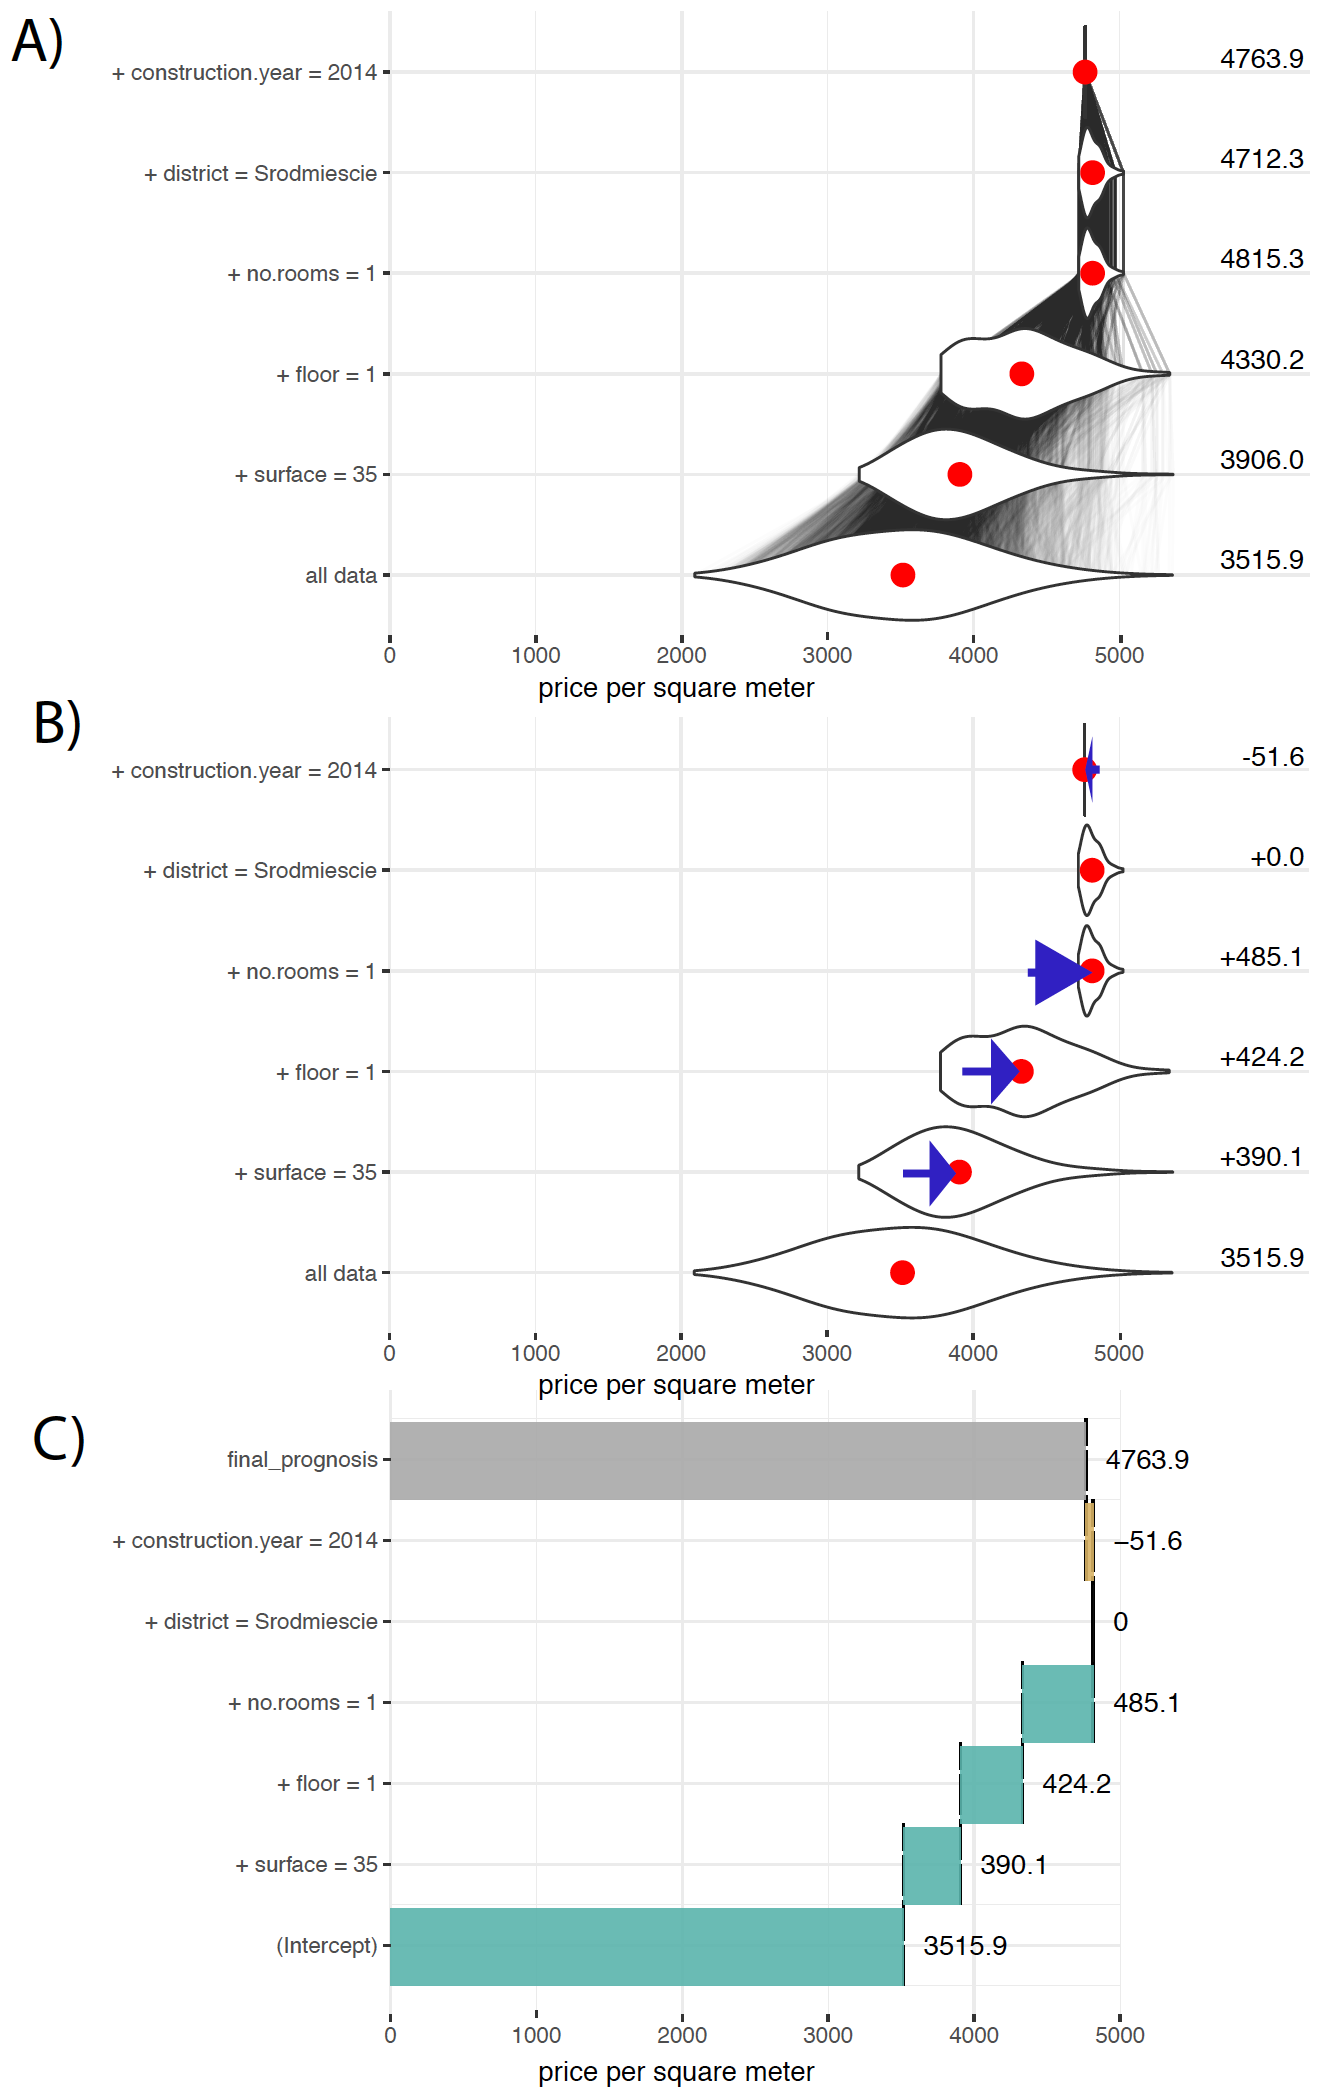
\includegraphics[width=0.7\linewidth]{figure/bd_price_4} 

}

\caption{(fig:BDPrice4) Break Down Plots show how variables move the model prediction from population average to the model prognosis for a single observation. A) TODO B) TODO C) TODO   An illustration of algorithm . Each row in this plot corresponds to a distribution of model scores $f(x)|x_IndSet = x^*_IndSet$ for different sets of $IndSet$ indexes. Initially $IndSet = 1, ..., p$ and in each step single variable is removed from this set. Labels on the left-hand side of the plots show which variable is removed in a given step. Red dots stand for conditional average - an estimate of relaxed predictions $f^{IndSet}(x^*)$. Violin plots summarize conditional distributions of scores while gray lines show how model predictions change for particular observations between consecutive relaxations. }\label{fig:BDPrice4}
\end{figure}

\hypertarget{how-to-construct-break-down-plots}{%
\section{How to construct Break Down
Plots}\label{how-to-construct-break-down-plots}}

Let us use the following notation:
\(x = (x_1, x_2, ..., x_d) \in \mathcal R^d\) is a vector with features.
\(f_M(x):R^{d} \rightarrow R\) is a model under consideration. It may be
a regression or classification model. Additionally \(X\) is a dataset
with \(n\) observations, this dataset will be used to learn joint
distribution of features.

For a single observation \(x\) the model prediction is equal to
\(f(x)\). Our goal is to attribute parts of this score to variables
(dimensions) in the \(R^{d}\) space.

\textbf{Model agnostic approach}

The intuition behind this approach is to identify components of \(x\)
that cannot be changed without a significant change in the prediction
\(f(x)\). In order to present this approach in a more formal way, we
first need to introduce some definitions.

\emph{Relaxed model prediction}

Let \(f^{IndSet}(x^{*})\) denotes an expected model prediction for
\(x^{*new*}\) relaxed on the set of indexes
\(IndSet \subset \{1, \ldots, p\}\).

\[
f^{IndSet}(x^{*}) = E[f(x)|x_{IndSet} = x^{*}_{IndSet}].
\]

Thus \(f^{IndSet}(x^{*})\) is an expected value for model response
conditioned on variables from set \(IndSet\) in such a way, that
\(\forall_{i\in IndSet} x_i = x^{*}_i\).

The intuition behind relaxed prediction is that we are interested in an
average model response for observations that are equal to \(x^{*}\) for
features from \(IndSet^C\) set and follow the population distribution
for features from \(IndSet\) set. Clearly, two extreme cases are

\[
f^{\{1, \ldots, p\}}(x^{*}) = f(x^{*}),
\] which is the case of no relaxation, and \[
f^{\emptyset}(x^{new}) = E [f(x)].
\] which corresponds to full relaxation.

We will say that a variable was relaxed, when we do not fix its value
and we let it follow the population distribution.

This will play a crucial part in the algorithm presented in this
section.

Since we do not know the joint distribution of \(x\), we will use its
estimate instead. \[
\widehat {f^{IndSet}(x^{*})} = \frac 1n \sum_{i = 1}^n f(x^i_{-IndSet},x^{*}_{IndSet}).
\] We will omit the dashes to simplify the notation.

\emph{Distance to relaxed model prediction}

Let us define the distance between model prediction and relaxed model
prediction for a set of indexes \(IndSet\).

\[
d(x^{*}, IndSet) := |f^{IndSet}(x^{*}) - f(x^{*})|.
\]

It is the difference between model prediction for observation \(x^{*}\)
and observation relaxed on features \(indSet\). The smaller the
difference, the less important are variables in the \(indSet\) set.

\emph{Added feature contribution}

For j-th feature we define its contribution relative to a set of indexes
\(IndSet\) (\emph{added contribution}) as

\[
\text{contribution}^{IndSet}(j) = f^{IndSet \cup \{j\}}(x^{*}) - f^{IndSet}(x^{*}).
\]

It is the change in model prediction for \(x^{*}\) after relaxation on
\(j\).

The model agnostic feature contribution is based on distances to relaxed
model predictions. In this approach we look for a series of variables
that can be relaxed in such a way so as to move model prediction from
\(f(x^{*})\) to a fully relaxed prediction \(E [f(x)]\) (expected value
for all model predictions). The order of features in this series is
important. But here we use a greedy strategy in which we add features to
the \(indSet\) iteratively (one feature per iteration) and minimize
locally the distance to relaxed model prediction.

The greedy search can start from a null set of indexes (then in each
step a single feature is being relaxed) or it can start from a full set
of relaxed features (then in each step a single feature is removed from
the set). The above approaches are called \emph{step-up} and
\emph{step-down}, respectively.

The algorithm \ref{alg:relaxedalg} presents the procedure that generates
a sequence of variables with increasing contributions. This sequence
corresponds to variables that can be relaxed in such a way so as to
minimize the distance to the original prediction. The resulting sequence
of \(Contributions\) and \(Variables\) may be plotted with Break Down
Plots. By relaxing consecutive variables one finds a path between single
prediction and average model prediction.

\textbf{Model agnostic break down of model predictions. The
\emph{step-down} approach.}

\begin{enumerate}
\def\labelenumi{\arabic{enumi}.}
\tightlist
\item
  \$p := \$ number of variables
\item
  \(IndSet := \{1, \ldots, p\}\), i.e.~set of indexes of all variables
\item
  FOR \(i \in \{1, \ldots, p\}\)
\item
  Find new variable that can be relaxed with small loss in relaxed
  distance to \(f(x^{*})\)
\item
  FOR \(j in IndSet\)
\item
  Calculate relaxed distance with \(j\) removed
\item
  \(dist(j) := d(x^{*}, IndSet \setminus \{j\})\)
\item
  END FOR 5.
\item
  Find and remove \(j\) that minimizes loss
\item
  \(j_{min} := \text{arg}\min_j dist(j)\)
\item
  \(Contribution^{IndSet}(i) := f^{IndSet}(x^{new}) - f^{IndSet \setminus \{j_{min}\}}(x^{*})\)
\item
  \(Variables(i) := j_{min}\)
\item
  \(IndSet := IndSet \setminus \{j_{min}\}\)
\item
  END FOR 3.
\end{enumerate}

\textbf{Approach for linear models}

For linear models (and also generalized linear models) the scoring
function (e.g.~link function) may be expressed as linear combination of
feature vectors.

\[
f(x^{*}) = (1, x^{*}) (\mu, \beta)^T = \mu + x^{*}_1 \beta_1 + \ldots + x^{*}_p \beta_p.
\]

In this case it is easy to attribute the impact of feature \(x_i\) to
prediction \(f(x^{*})\). The most straightforward approach would be to
use the \(x^{*}_i \beta_i\) as the attribution. However, it is easier to
interpret variable attributions if they are invariant to scale-location
transformations of \(x_i\), such as change of the unit or origin. This
is why for linear models the variable attributions are defined as
\((x^{*}_i - \bar x_i) \beta_i\).

Previous equation may be rewritten as follows:

\[
f(x^{*}) = (1, x^{*}) (\mu, \beta)^T = baseline + (x^{*}_1 - \bar x_1) \beta_1 + ... + (x^{*}_p - \bar x_p) \beta_p
\]

where

\[
baseline = \mu + \bar x_1 \beta_1 + ... + \bar x_p \beta_p.
\]

Components \((x^{*}_i - \bar x_i) \beta_i\) are all expressed in the
same units.

\hypertarget{interactions}{%
\section{Interactions}\label{interactions}}

\begin{figure}

{\centering 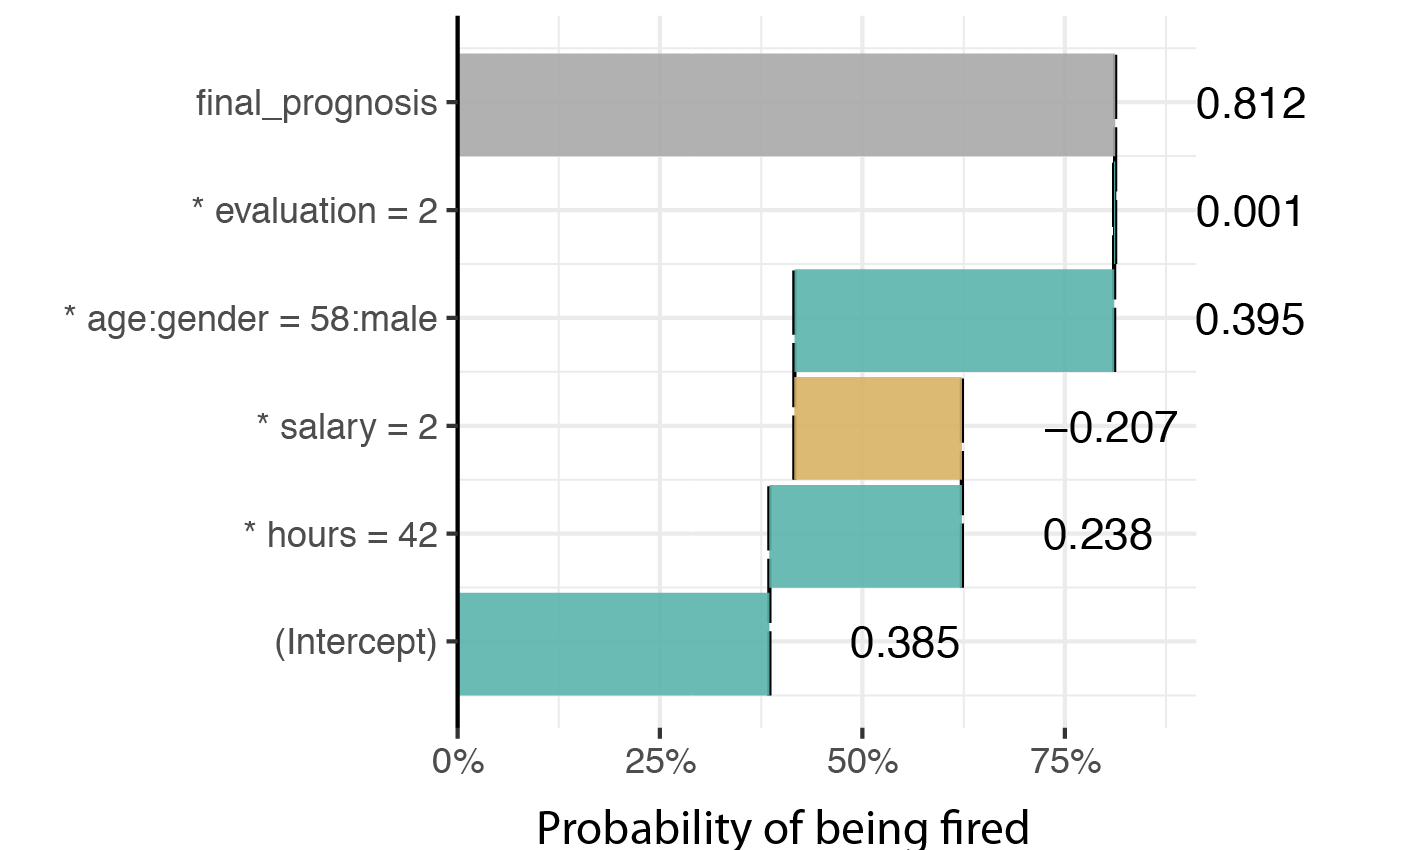
\includegraphics[width=0.7\linewidth]{figure/bd_inter_1} 

}

\caption{(fig:bdInter1) Break Down plot with interactions }\label{fig:bdInter1}
\end{figure}

\hypertarget{pros-and-cons}{%
\section{Pros and cons}\label{pros-and-cons}}

Break Down Plots gives a uniform approach to decompose model prediction
into parts that can be attributed additively to variables. Below we
summarize key strengths and weaknesses of this approach.

\textbf{Pros}

\begin{itemize}
\tightlist
\item
  Graphical representation of Break Down plots is easy to understand.
\item
  Break Down plots are compact, many variables may be presented in a
  small space.
\item
  Break Down plots are model agnostic yet they reduce to intuitive
  interpretation for linear Gaussian and generalized models.
\item
  Break Down plots are faster than other approaches to variable
  attribution.
\end{itemize}

\textbf{Cons}

\begin{itemize}
\tightlist
\item
  If the model is non-additive then showing only additive contributions
  may be misleading.
\item
  For large number of variables the Break Down plot may be messy with
  many variables having small contributions.
\item
  For non-additive models the Break Down plot will depend on the order
  of variables being relaxed.
\end{itemize}

\hypertarget{code-snippets-for-r}{%
\section{Code snippets for R}\label{code-snippets-for-r}}

In this section we present key features of the \texttt{breakDown}
package for R \citep{R-breakDown}. This package covers all features
presented in this chapter. It is available on CRAN and GitHub. Find more
examples at the website of this package
\texttt{https://pbiecek.github.io/breakDown/}.

\textbf{Model preparation}

In this section we will present examples based on the
\texttt{apartments} dataset. See section TODO for more details.

\begin{Shaded}
\begin{Highlighting}[]
\KeywordTok{library}\NormalTok{(}\StringTok{"DALEX"}\NormalTok{)}
\KeywordTok{head}\NormalTok{(HR)}
\end{Highlighting}
\end{Shaded}

\begin{verbatim}
##   gender      age    hours evaluation salary   status
## 1   male 32.58267 41.88626          3      1    fired
## 2 female 41.21104 36.34339          2      5    fired
## 3   male 37.70516 36.81718          3      0    fired
## 4 female 30.06051 38.96032          3      2    fired
## 5   male 21.10283 62.15464          5      3 promoted
## 6   male 40.11812 69.53973          2      0    fired
\end{verbatim}

The problem here is to predict average price for square meter for an
apartment. Let's build a random forest model with \texttt{randomForest}
package \citep{R-randomForest}.

\begin{Shaded}
\begin{Highlighting}[]
\KeywordTok{library}\NormalTok{(}\StringTok{"randomForest"}\NormalTok{)}
\NormalTok{model <-}\StringTok{ }\KeywordTok{randomForest}\NormalTok{(status }\OperatorTok{~}\StringTok{ }\NormalTok{gender }\OperatorTok{+}\StringTok{ }\NormalTok{age }\OperatorTok{+}\StringTok{ }\NormalTok{hours }\OperatorTok{+}\StringTok{ }\NormalTok{evaluation }\OperatorTok{+}\StringTok{ }\NormalTok{salary, }\DataTypeTok{data =}\NormalTok{ HR)}
\NormalTok{model}
\end{Highlighting}
\end{Shaded}

\begin{verbatim}
## 
## Call:
##  randomForest(formula = status ~ gender + age + hours + evaluation +      salary, data = HR) 
##                Type of random forest: classification
##                      Number of trees: 500
## No. of variables tried at each split: 2
## 
##         OOB estimate of  error rate: 27.27%
## Confusion matrix:
##          fired   ok promoted class.error
## fired     2276  382      197   0.2028021
## ok         532 1253      436   0.4358397
## promoted   205  388     2178   0.2140022
\end{verbatim}

Model exploration with \texttt{breakDown} package is performed in three
steps.

\textbf{1. Create an explainer - wrapper around model and validation
data.}

Since all other functions work in a model agnostic fashion, first we
need to define a wrapper around the model. Here we are using the
\texttt{explain()} function from \texttt{DALEX} package \citep{R-DALEX}.

\begin{Shaded}
\begin{Highlighting}[]
\NormalTok{explainer_rf_fired <-}\StringTok{ }\KeywordTok{explain}\NormalTok{(model,}
                 \DataTypeTok{data =}\NormalTok{ HR,}
                 \DataTypeTok{y =}\NormalTok{ HR}\OperatorTok{$}\NormalTok{status }\OperatorTok{==}\StringTok{ "fired"}\NormalTok{,}
                 \DataTypeTok{predict_function =} \ControlFlowTok{function}\NormalTok{(m,x) }\KeywordTok{predict}\NormalTok{(m,x, }\DataTypeTok{type =} \StringTok{"prob"}\NormalTok{)[,}\DecValTok{1}\NormalTok{],}
                 \DataTypeTok{label =} \StringTok{"fired"}\NormalTok{)}
\end{Highlighting}
\end{Shaded}

\textbf{2. Define point of interest.}

Break Down Plots decompose model prediction around a single point.

\begin{Shaded}
\begin{Highlighting}[]
\NormalTok{new_observation <-}\StringTok{ }\KeywordTok{data.frame}\NormalTok{(}\DataTypeTok{gender =} \KeywordTok{factor}\NormalTok{(}\StringTok{"male"}\NormalTok{, }\DataTypeTok{levels =} \KeywordTok{c}\NormalTok{(}\StringTok{"male"}\NormalTok{, }\StringTok{"female"}\NormalTok{)),}
                      \DataTypeTok{age =} \FloatTok{57.7}\NormalTok{,}
                      \DataTypeTok{hours =} \FloatTok{42.3}\NormalTok{,}
                      \DataTypeTok{evaluation =} \DecValTok{2}\NormalTok{,}
                      \DataTypeTok{salary =} \DecValTok{2}\NormalTok{)}

\KeywordTok{predict}\NormalTok{(model, new_observation, }\DataTypeTok{type =} \StringTok{"prob"}\NormalTok{)}
\end{Highlighting}
\end{Shaded}

\begin{verbatim}
##   fired    ok promoted
## 1 0.778 0.218    0.004
## attr(,"class")
## [1] "matrix" "votes"
\end{verbatim}

\textbf{3. Calculate BD decomposition}

The \texttt{break\_down()} function calculates BP decomposition for
selected model around selected observation.

The result from \texttt{break\_down()} function is a data frame with
variable attributions.

\begin{Shaded}
\begin{Highlighting}[]
\KeywordTok{library}\NormalTok{(}\StringTok{"breakDown"}\NormalTok{)}
\NormalTok{bd_rf <-}\StringTok{ }\KeywordTok{break_down}\NormalTok{(explainer_rf_fired,}
\NormalTok{                 new_observation,}
                 \DataTypeTok{keep_distributions =} \OtherTok{TRUE}\NormalTok{)}

\NormalTok{bd_rf}
\end{Highlighting}
\end{Shaded}

\begin{verbatim}
##                        contribution
## (Intercept)                   0.376
## * hours = 42                  0.240
## * salary = 2                 -0.202
## * age:gender = 58:male        0.398
## * evaluation = 2             -0.034
## final_prognosis               0.778
## baseline:  0
\end{verbatim}

\begin{Shaded}
\begin{Highlighting}[]
\KeywordTok{plot}\NormalTok{(bd_rf) }
\end{Highlighting}
\end{Shaded}

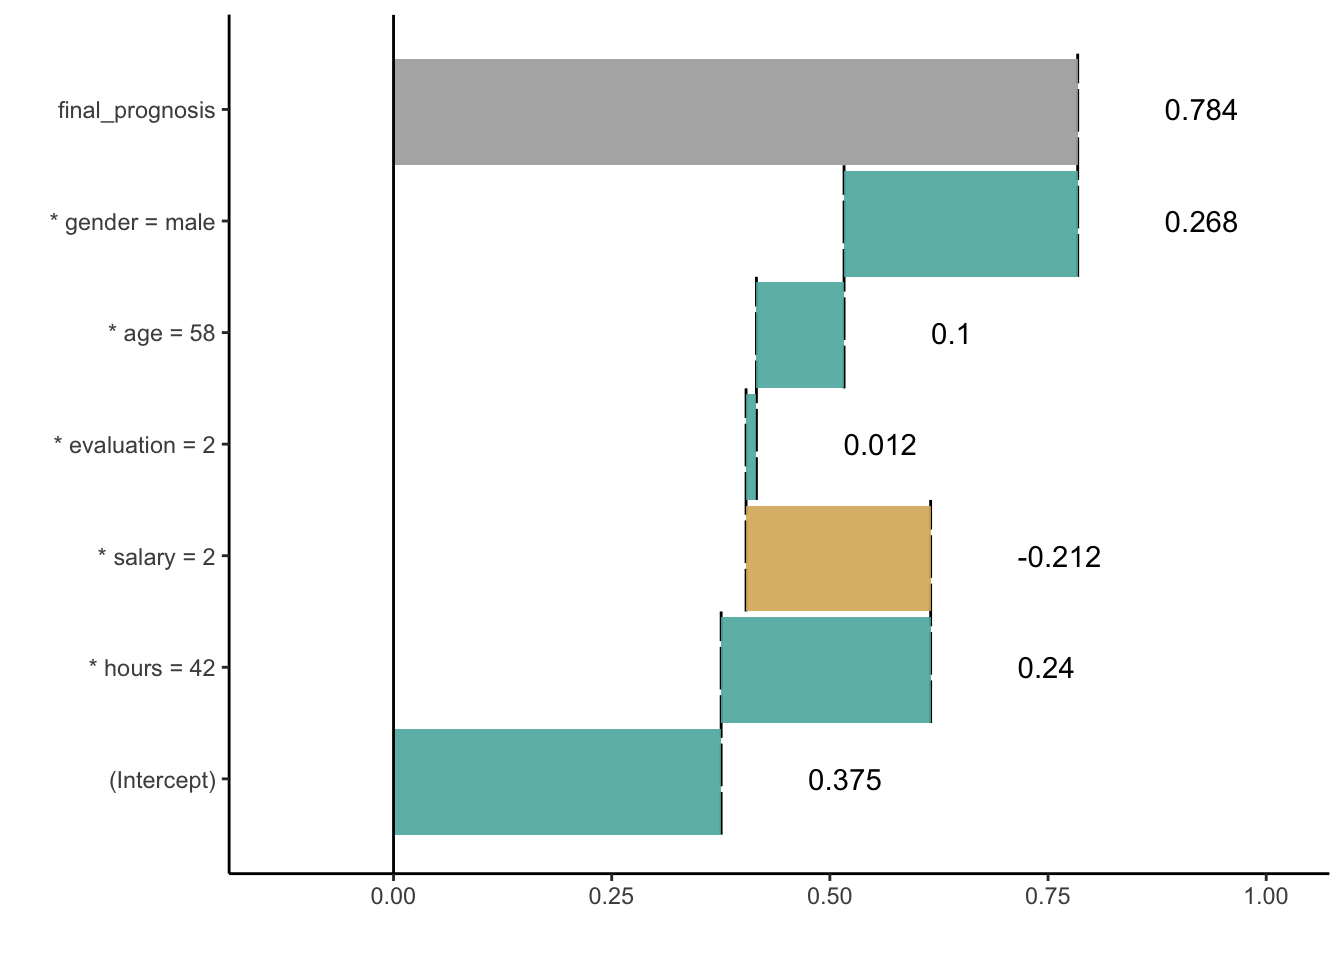
\includegraphics{PM_VEE_files/figure-latex/unnamed-chunk-7-1.pdf}

\begin{Shaded}
\begin{Highlighting}[]
\KeywordTok{plot}\NormalTok{(bd_rf, }\DataTypeTok{plot_distributions =} \OtherTok{TRUE}\NormalTok{) }
\end{Highlighting}
\end{Shaded}

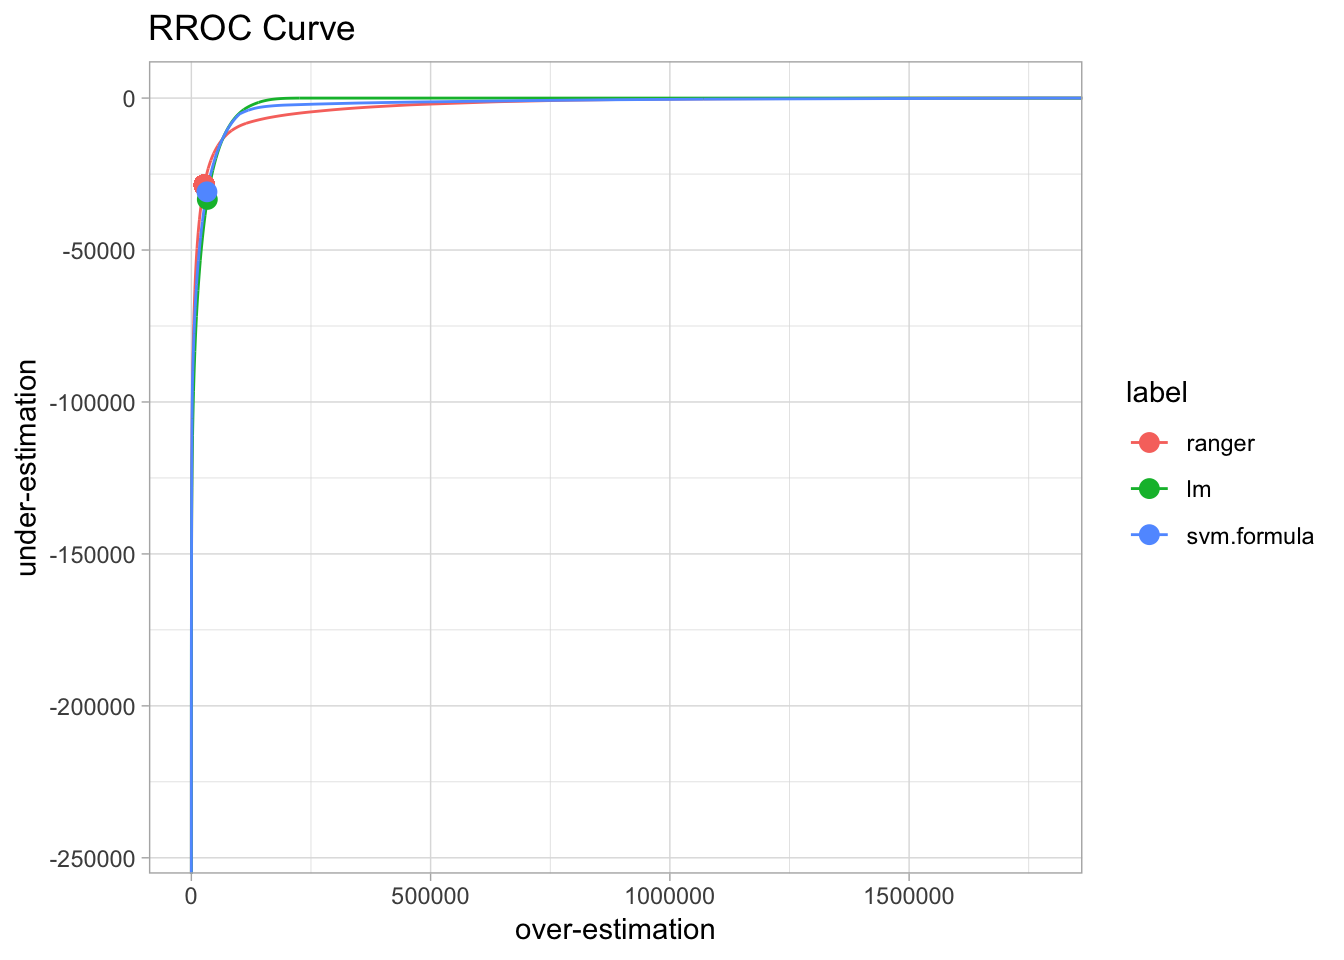
\includegraphics{PM_VEE_files/figure-latex/unnamed-chunk-7-2.pdf}

\hypertarget{shapley}{%
\chapter{Shapley Values}\label{shapley}}

Variable Atribution

This approach can be seen as an approximation of Shapley values where
feature contribution is linked with the average effect of a feature
across all possible relaxations. These approaches are identical for
additive models. For non-additive models the additive attribution is
just an approximation in both cases, yet the greedy strategy produces
explanations that are easier to interpret. It is worth noting that
similar decomposition of predictions and measures of contribution for
classifiers have been examined in \cite{4407709}.

\hypertarget{LIME}{%
\chapter{LIME: Local Interpretable Model-Agnostic
Explanations}\label{LIME}}

\citep{R-lime} \citep{R-live}

\begin{Shaded}
\begin{Highlighting}[]
\KeywordTok{library}\NormalTok{(lime)}
\KeywordTok{library}\NormalTok{(live)}
\end{Highlighting}
\end{Shaded}

Sparse model approximation / variable selection / feature ranking

live: Local Interpretable (Model-Agnostic) Visual Explanations

\hypertarget{ceterisParibus}{%
\chapter{Ceteris Paribus Principle}\label{ceterisParibus}}

In this section we introduce tools based on Ceteris Paribus principle.
The main goal for these tools is to help understand how changes in model
input affect changes in model output.

Presented explainers are linked with the second law introduced in
Section \ref{three-single-laws}, i.e.~law for prediction's speculations.
This is why these explainers are also known as \emph{What-If model
analysis} or \emph{Individual Conditional EXpectations} \citep{ICEbox}.
It turns out that it is easier to understand how blacx-box model is
working if we can play with it by changing variable by variable.

Think of following usecases:

\begin{itemize}
\tightlist
\item
  Think about a model for hart attack. How the model response would
  change if a patient cuts the number of smoked cigarettes by half or
  increase physical activity.
\item
  Think about a model for credit scoring. A customer gets a low score
  and is asking what he needs to change to increase this score to a
  certain level, to pass the bank criteria.
\item
  Think about a model for apartment prices. An investor wants to know
  how much the price may increase if apartment standard is upgraded.
\end{itemize}

\hypertarget{introduction-2}{%
\section{Introduction}\label{introduction-2}}

\emph{Ceteris paribus} is a Latin phrase meaning ``other things held
constant'' or ``all else unchanged''. Using this principle we examine
input variable per variable separatly, asumming that effects of all
other variables are unchanged. See Figure
\ref{fig:modelResponseCurveLine}

\begin{figure}

{\centering 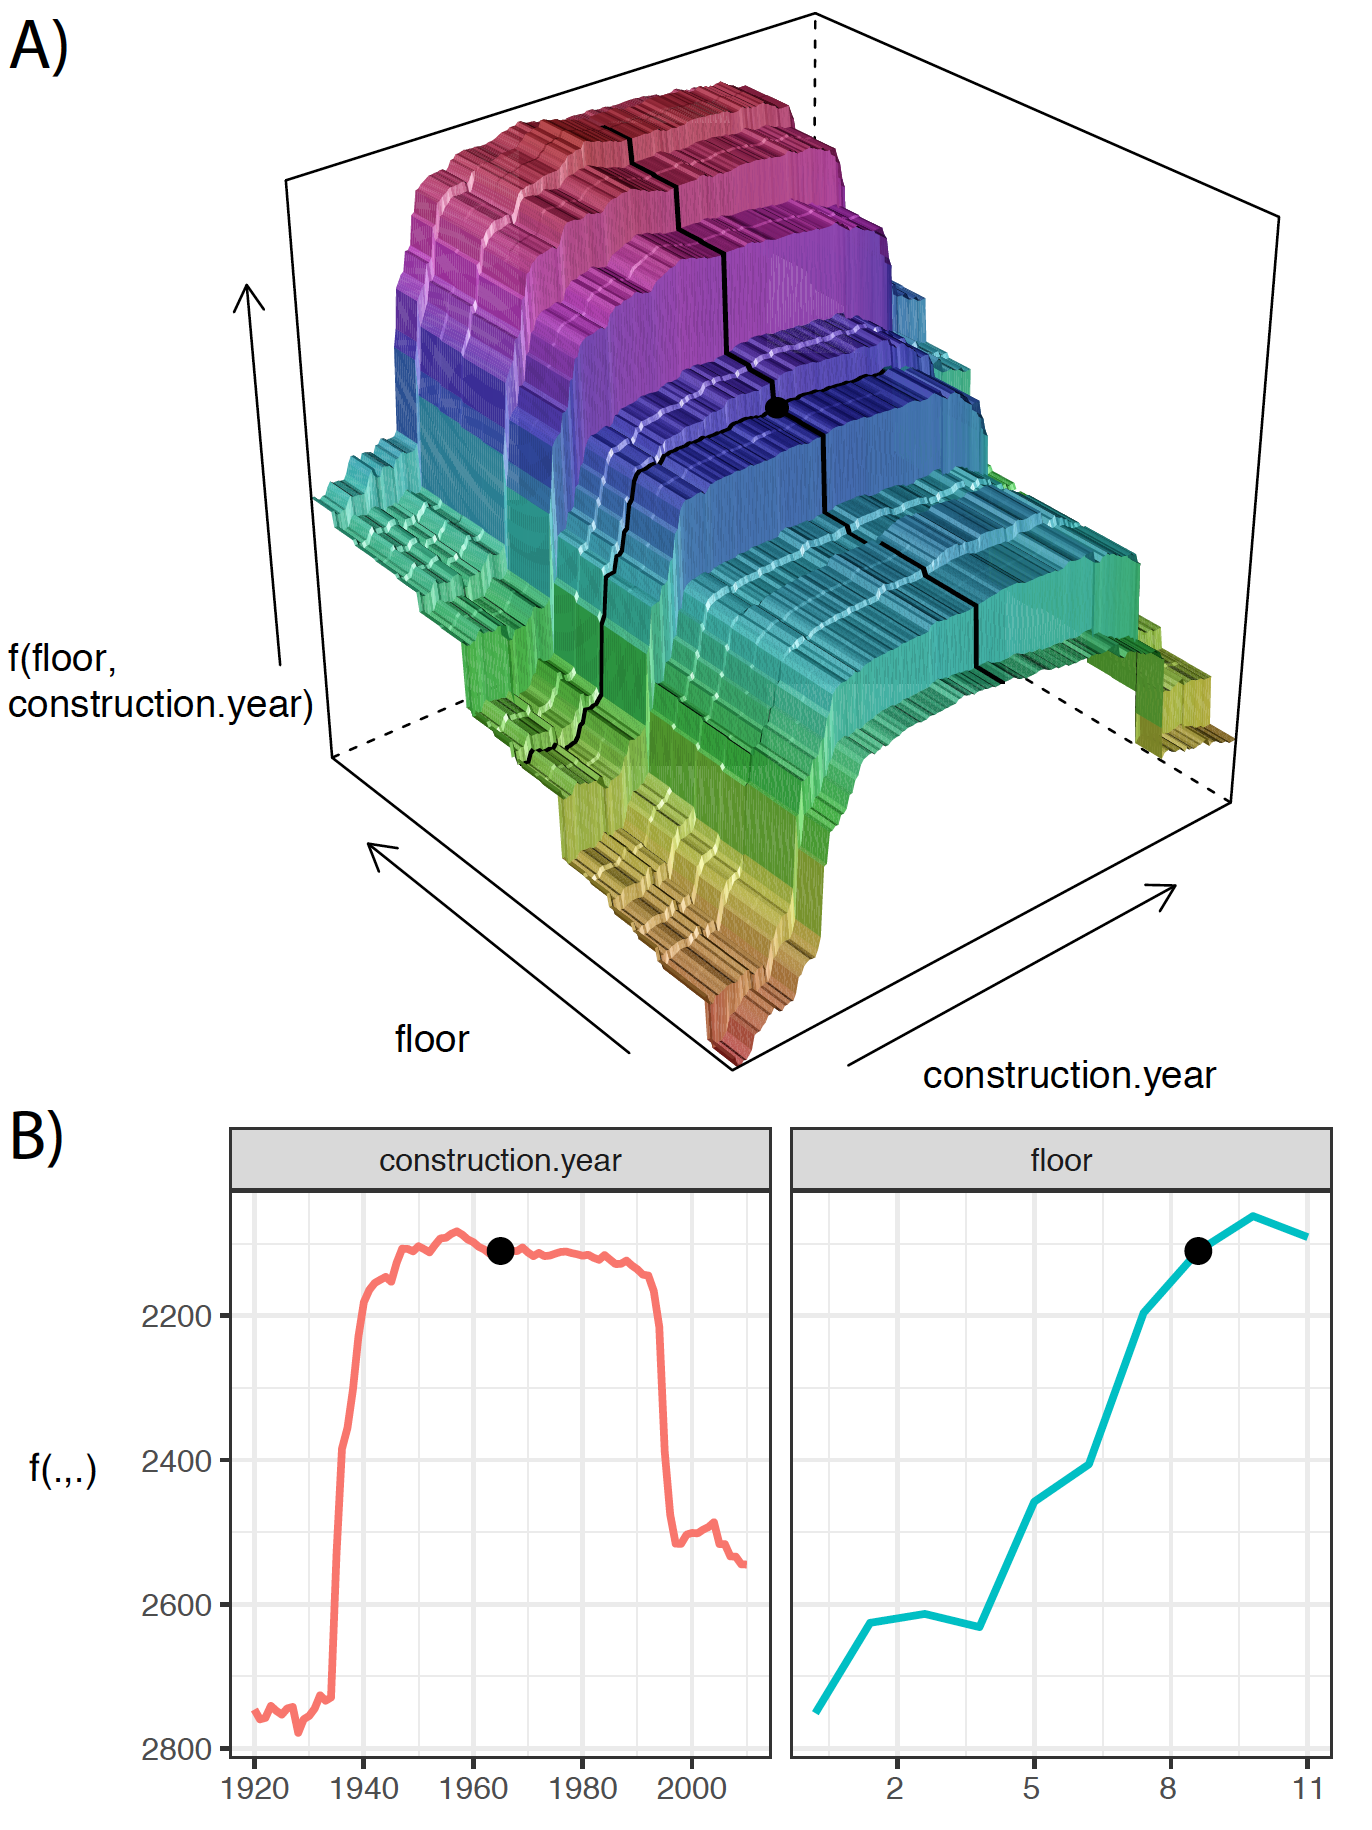
\includegraphics[width=0.7\linewidth]{figure/model_response_line} 

}

\caption{(fig:modelResponseCurveLine) A) Model response surface. Ceteris Paribus profiles marked with black curves helps to understand the curvature of the model response by updating only a single variable. B) CP profiles are individual conditional model responses}\label{fig:modelResponseCurveLine}
\end{figure}

Similar to the LIME method introduced in the section \ref{LIME}, Ceteris
Paribus profiles examine curvature of a model response function. The
difference between these two methods that LIME approximates the model
curvature with a simpler white-box model that is easier to present.
Usually the LIME model is sparse, thus our attention may be limited to
smaller number of dimensions. In contrary, the CP plots show conditional
model response for every variable. In the last subsection we discuss
pros and cons of this approach.

\hypertarget{ceterisParibus1d}{%
\section{1D profiles}\label{ceterisParibus1d}}

Let \(f_{M}(x): \mathcal R^{d} \rightarrow \mathcal R\) denote a
predictive model, i.e.~function that takes \(d\) dimensional vector and
calculate numerical score. Symbol \(x \in \mathcal R^d\) refers to a
point in the feature space. We use subscript \(x_i\) to refer to a
different data points and superscript \(x^j\) to refer to specific
dimensions. Additionally, let \(x^{-j}\) denote all coordinates except
\(j\)-th and let \(x|^j=z\) denote a data point \(x^*\) with all
coordinates equal to \(x\) except coordinate \(j\) equal to value \(z\).
I.e. \(\forall_{i \neq {j}} x^i = x^{*,i}\) and \(x^j = z\). In other
words \(x|^j=z\) denote a \(x\) with \(j\)th coordinate changed to
\(z\).

Now we can define uni-dimensional Ceteris Paribus Profile for model
\(f\), variable \(j\) and point \(x\) as

\[
CP^{f, j, x}(z) := f(x|^j = z).
\] I.e. CP profile is a model response obtained for observations created
based on \(x\) with coordinate \(j\) changed and all other coordinates
kept unchanged.

A natural way to visualise CP profiles is to use a profile plot as in
Figure \ref{fig:HRCPFiredHours}.

Figure \ref{fig:HRCPFiredHours} shows an example of Ceteris Paribus
profile. The black dot stands for prediction for a single observation.
Grey line show how the model response would change if in this single
observation coordinate \texttt{hours} will be changed to selected value.
One thing that we can read is that the model response is not smooth and
there is some variability along the profile. Second thing is that for
this particular observation the model response would drop significantly
if the variable \texttt{hours} will be higher than 45.

\begin{figure}

{\centering 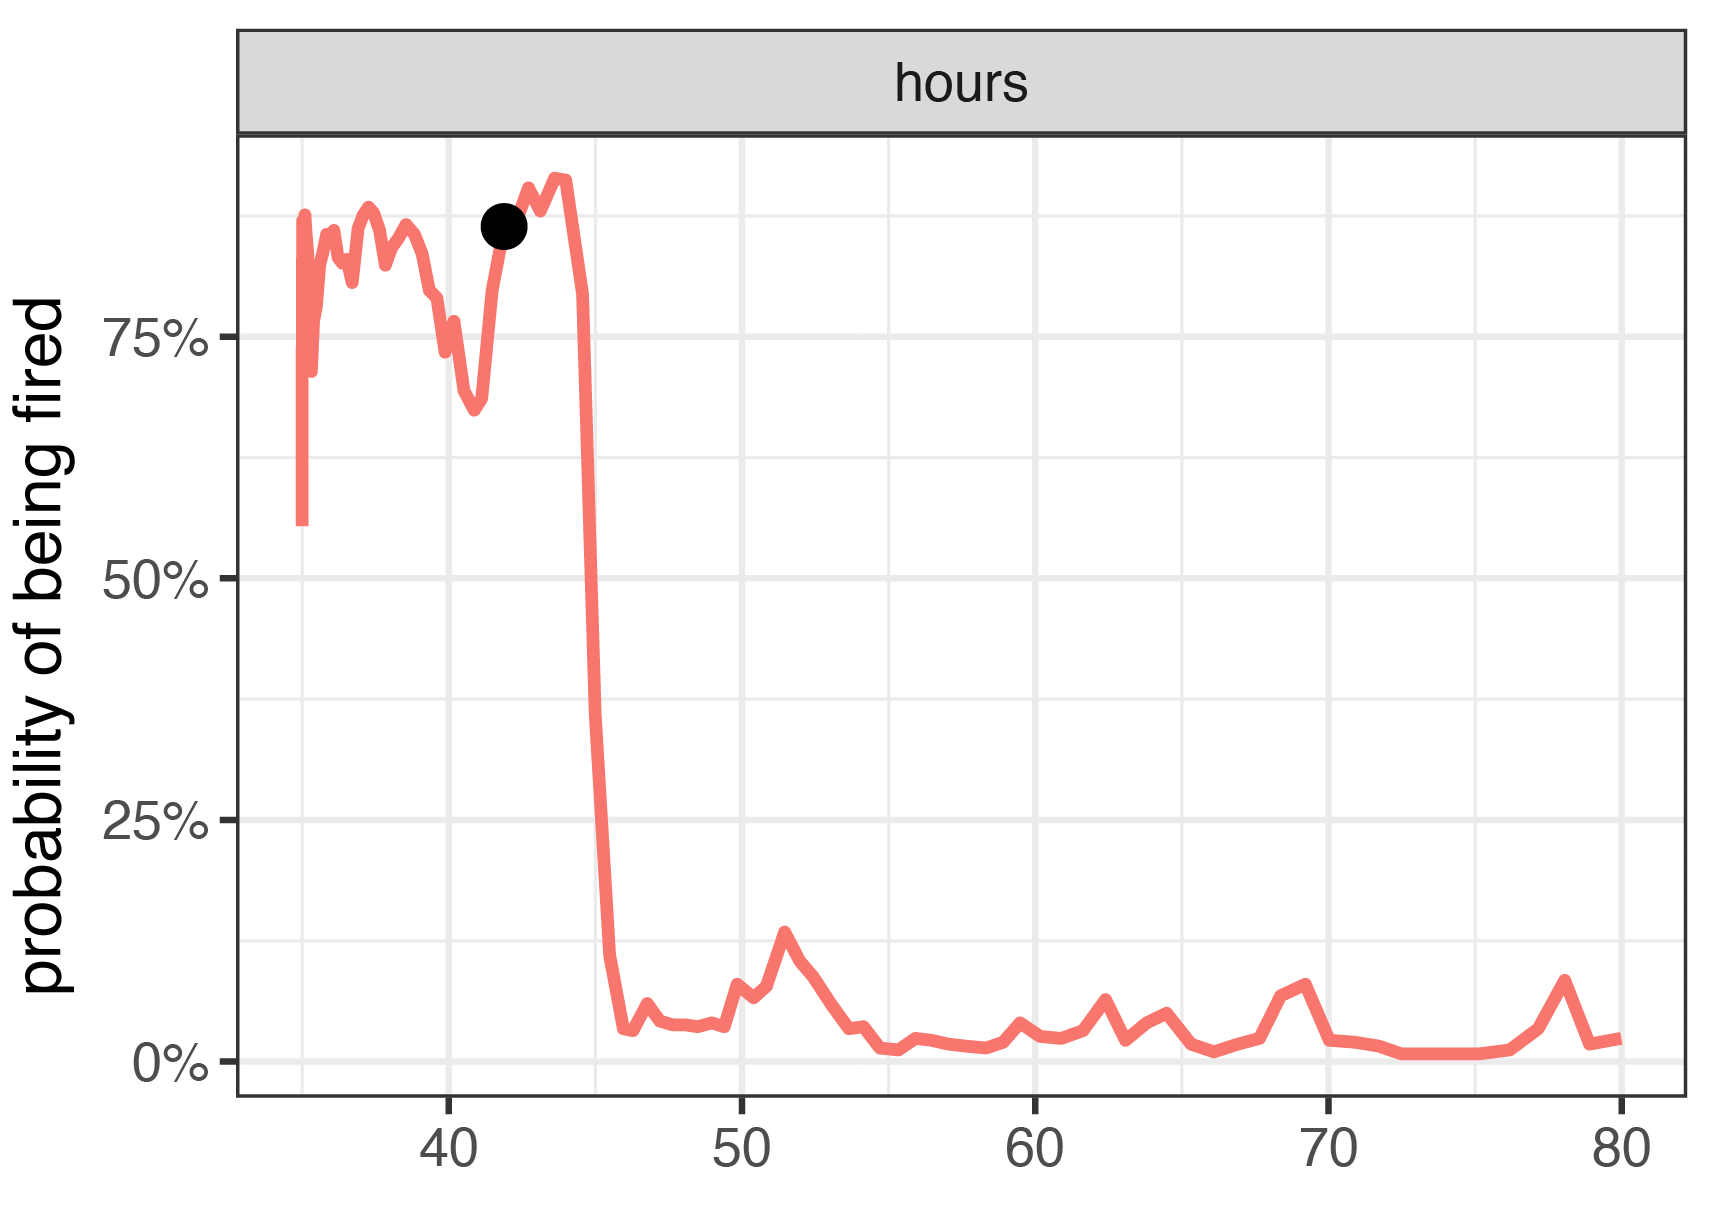
\includegraphics[width=0.5\linewidth]{figure/HR_cp_fired_hours} 

}

\caption{(fig:HRCPHiredHours) Ceteris Paribus profile for Random Forest model that assess the probability of being fired in call center as a function of average number of working hours}\label{fig:HRCPFiredHours}
\end{figure}

Since in the example dataset we are struggling with model for three
classes, one can plot CP profiles for each class in the same panel. See
an example in the Figure \ref{fig:HRCPAllHours}.

\begin{figure}

{\centering 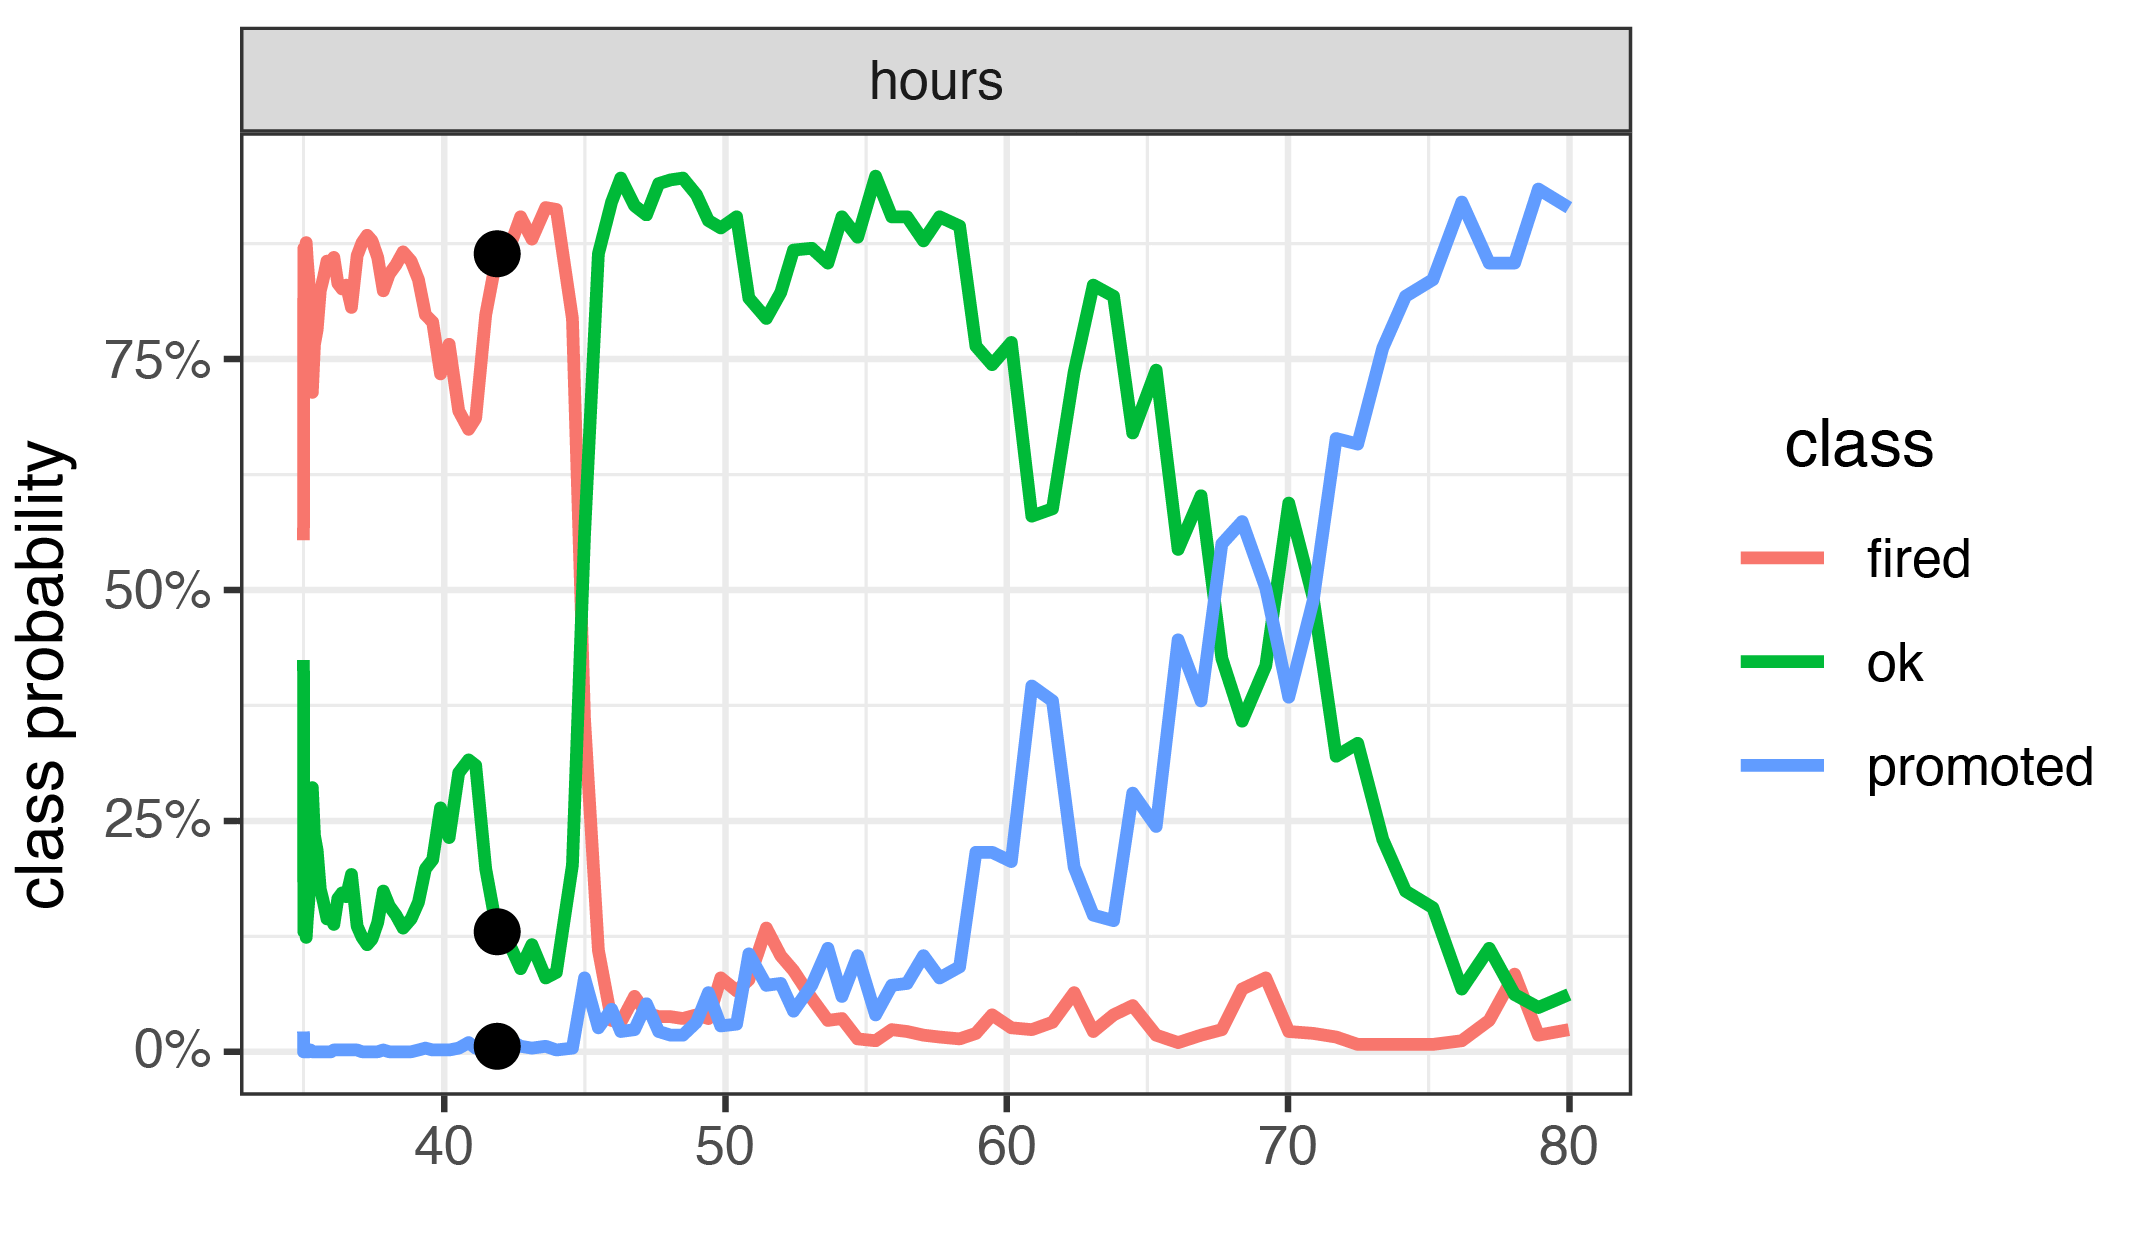
\includegraphics[width=0.6\linewidth]{figure/HR_cp_all_hours} 

}

\caption{(fig:HRCPAllHours) Ceteris Paribus profiles for three classess predicted by the Random Forest model as a function of average number of working hours}\label{fig:HRCPAllHours}
\end{figure}

Usually model input consist many variables, then it is beneficial to
show more variables at the same time. The easiest way to do so is to
plot consecutive variables on separate panels. See an example in Figure
\ref{fig:HRCPFiredAll}.

\begin{figure}

{\centering 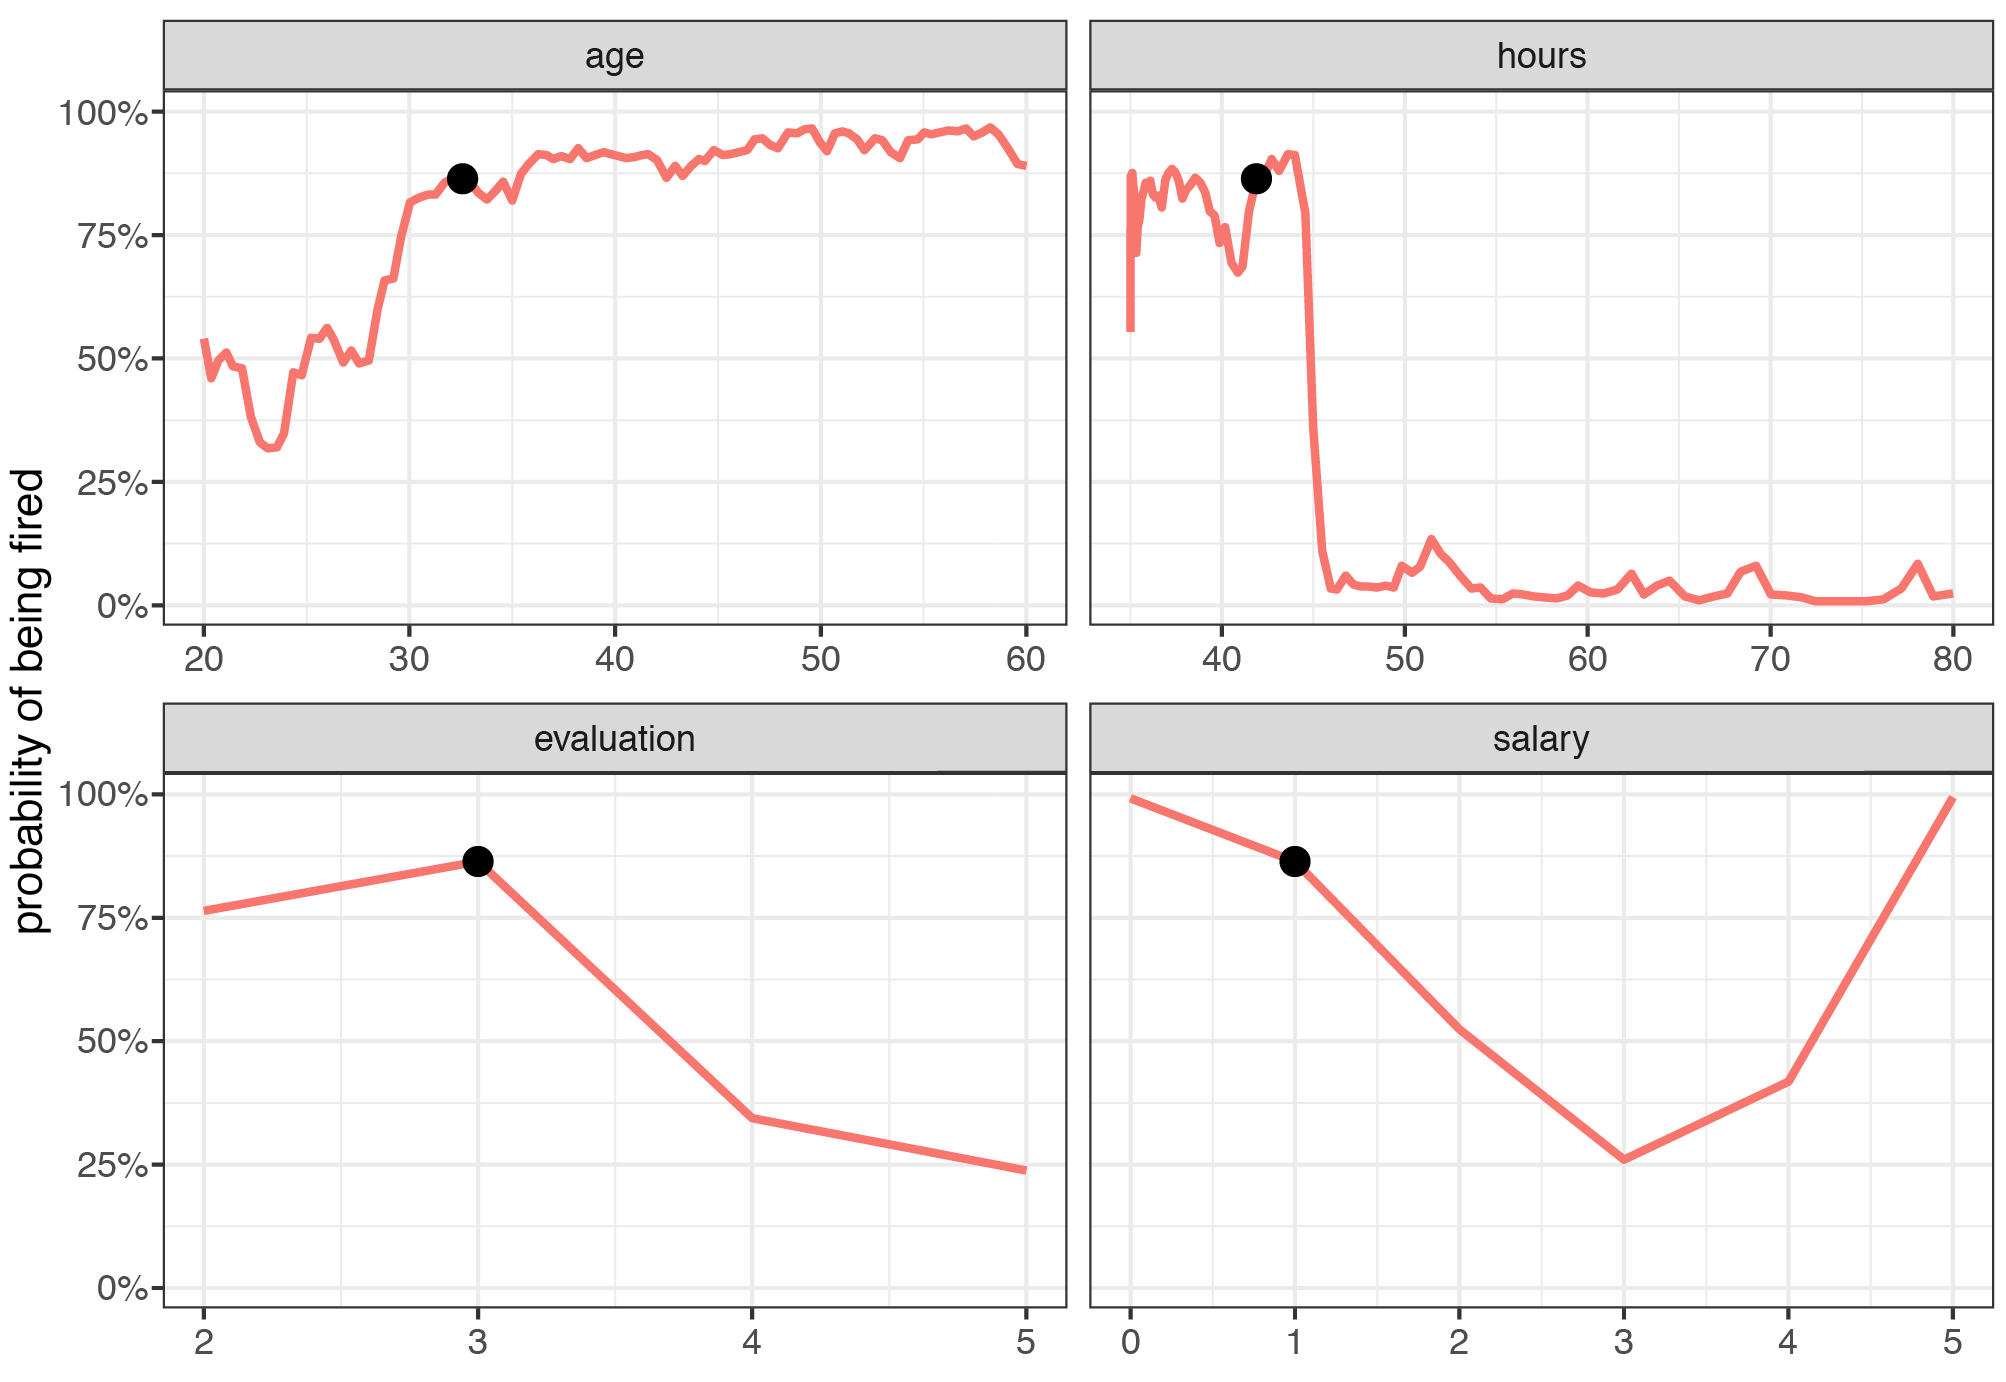
\includegraphics[width=0.7\linewidth]{figure/HR_cp_fired_all} 

}

\caption{(fig:HRCPFiredAll) Ceteris Paribus profiles for all continuous variables}\label{fig:HRCPFiredAll}
\end{figure}

\hypertarget{oscillations}{%
\section{Profile oscillations}\label{oscillations}}

Visual examination of variables is insightful, but for large number of
variables we end up with large number of panels, most of which are flat.
This is why we want to asses variable importance and show only profiles
for important variables. The advantage of CP profiles is that they lead
to a very natural and intuitive way of assessing the variable importance
for a single prediction. The intuition is: the more important variable
the larger are changes along the CP profile. If variable is not
important then model response will barely change. If variable is
important the CP profile change a lot for different values of a
variable.

Let's write it down in a more formal way.

Let \(vip^{CP}_j(x)\) denotes variable importance calculated based on CP
profiles in point \(x\) for variable \(j\).

\[
vip^{CP}_j(x) = \int_{-\inf}^{inf} |CP^{f,j,x}(z) - f(x)| dz
\]

So it's an absolute deviation from \(f(x)\). Note that one can consider
different modification of this coefficient:

\begin{enumerate}
\def\labelenumi{\arabic{enumi}.}
\tightlist
\item
  Deviations can be calculated not as a distance from \(f(x)\) but from
  average \(\bar CP^{f,j,x}(z)\).
\item
  The integral may be weighted based on the density of variable \(x^j\).
\item
  Instead of absolute deviations one may use root from average squares.
\end{enumerate}

TODO: we need to verify which approach is better. Anna Kozak is working
on this

The straightforward estimator for \(vip^{CP}_j(x)\) is

\[
\widehat{ vip^{CP}_j(x)} = \frac 1n \sum_{i=1}^n |CP^{f,j,x}(x_i) - f(x)|.
\]

Figure \ref{fig:CPVIPprofiles} shows the idea behind measuring
oscillations. The larger the highlighted area the more important is the
variable.

\begin{figure}

{\centering 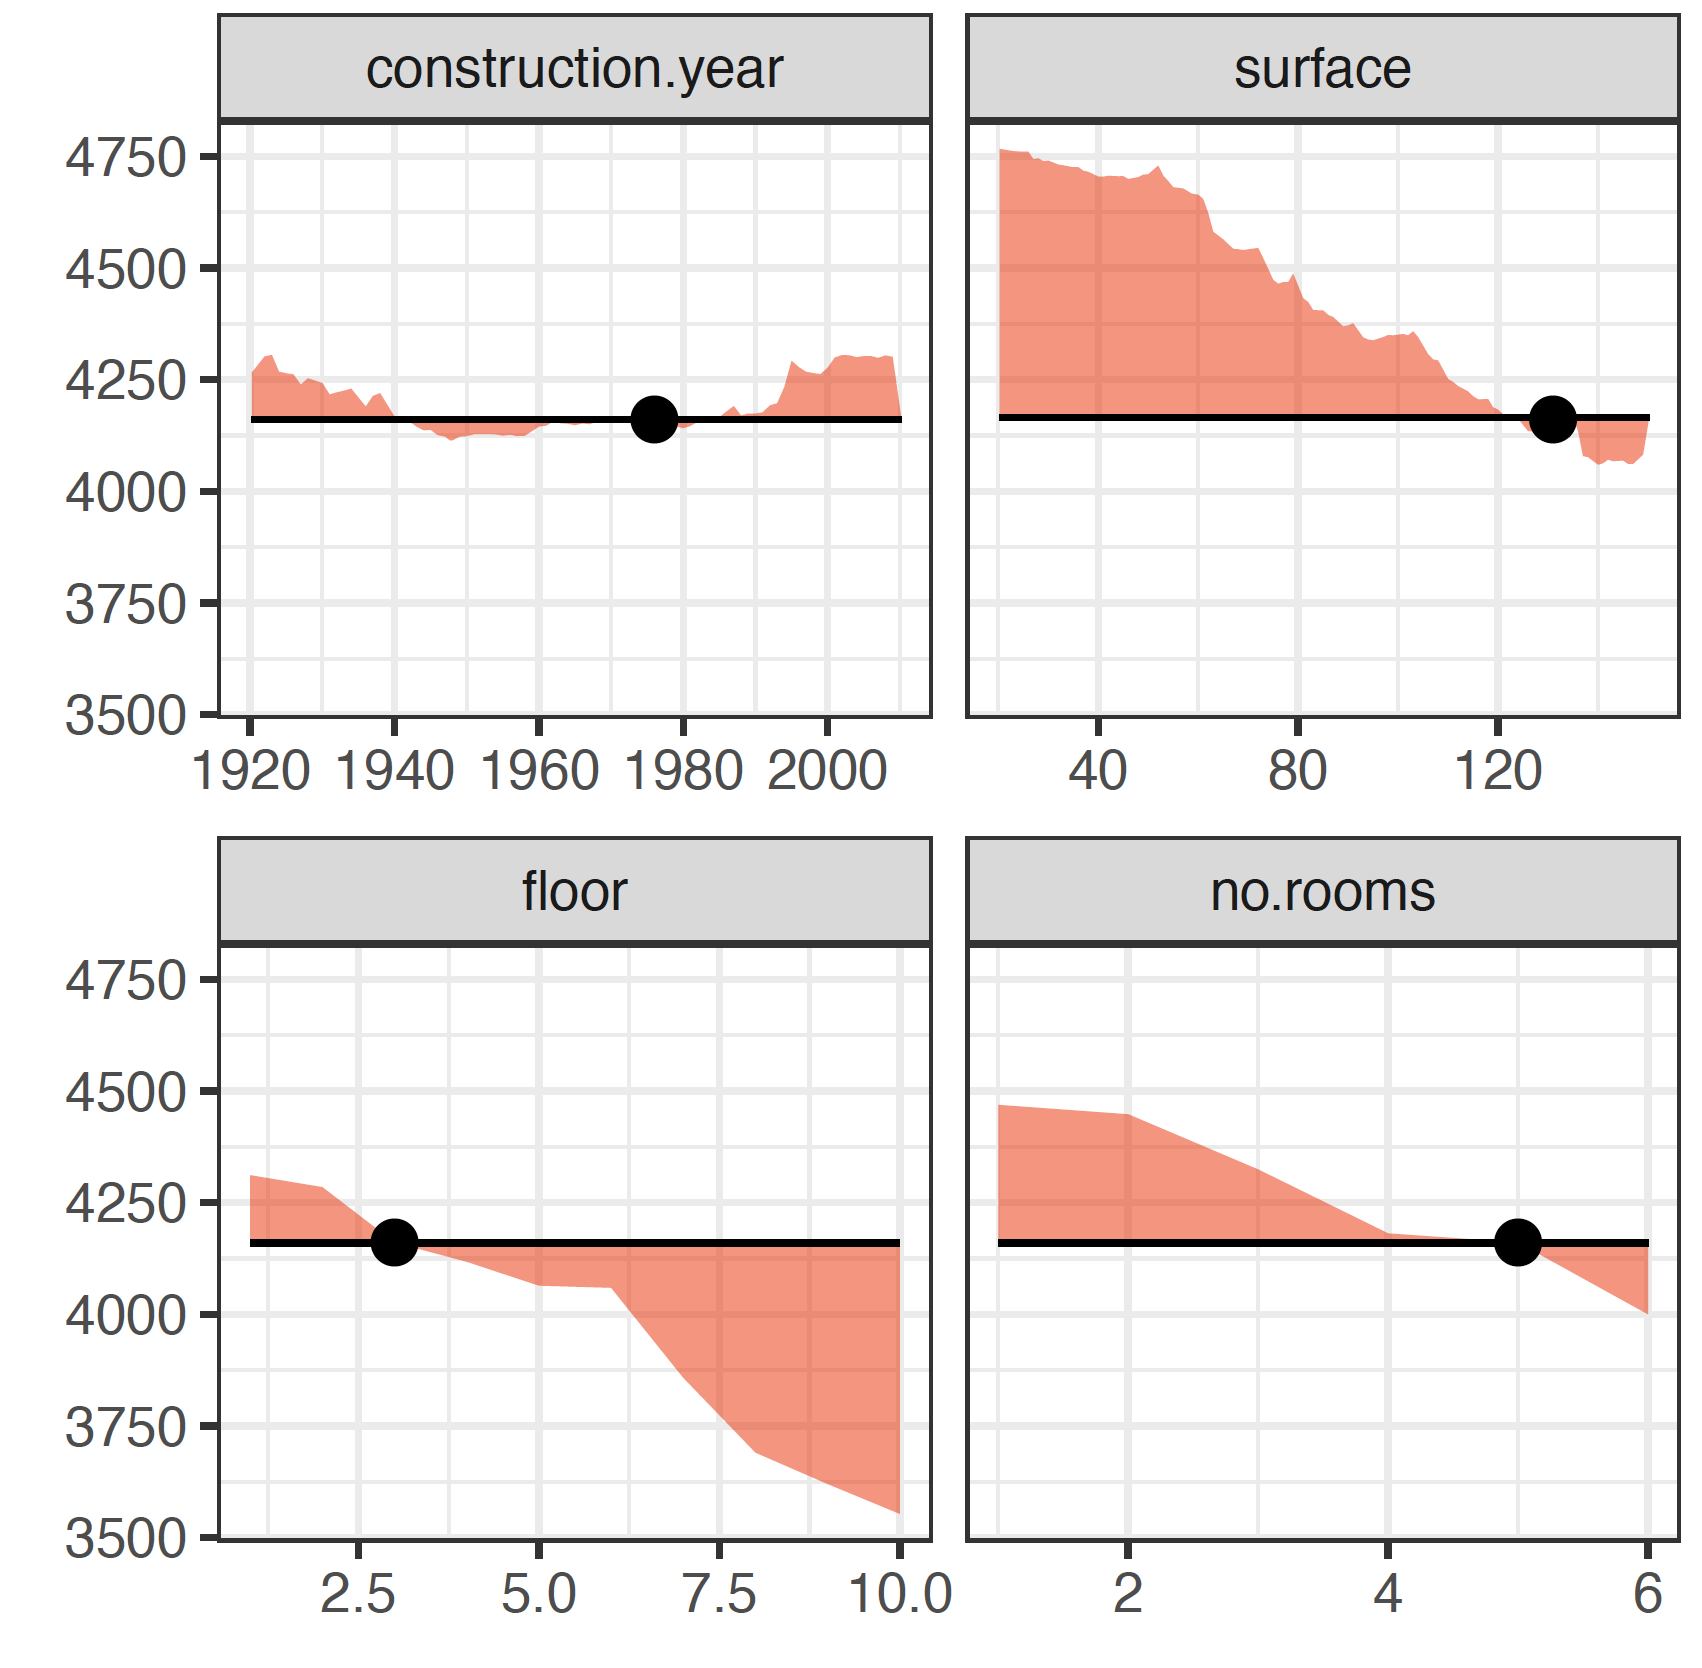
\includegraphics[width=0.5\linewidth]{figure/CP_VIP_profiles} 

}

\caption{(fig:CPVIPprofiles) CP oscillations are average deviations between CP profiles and the model response}\label{fig:CPVIPprofiles}
\end{figure}

Figure \ref{fig:CPVIP1} summarizes variable oscillations. Such visuals
help to quickly grasp how large are model oscillations around a specific
point.

\begin{figure}

{\centering 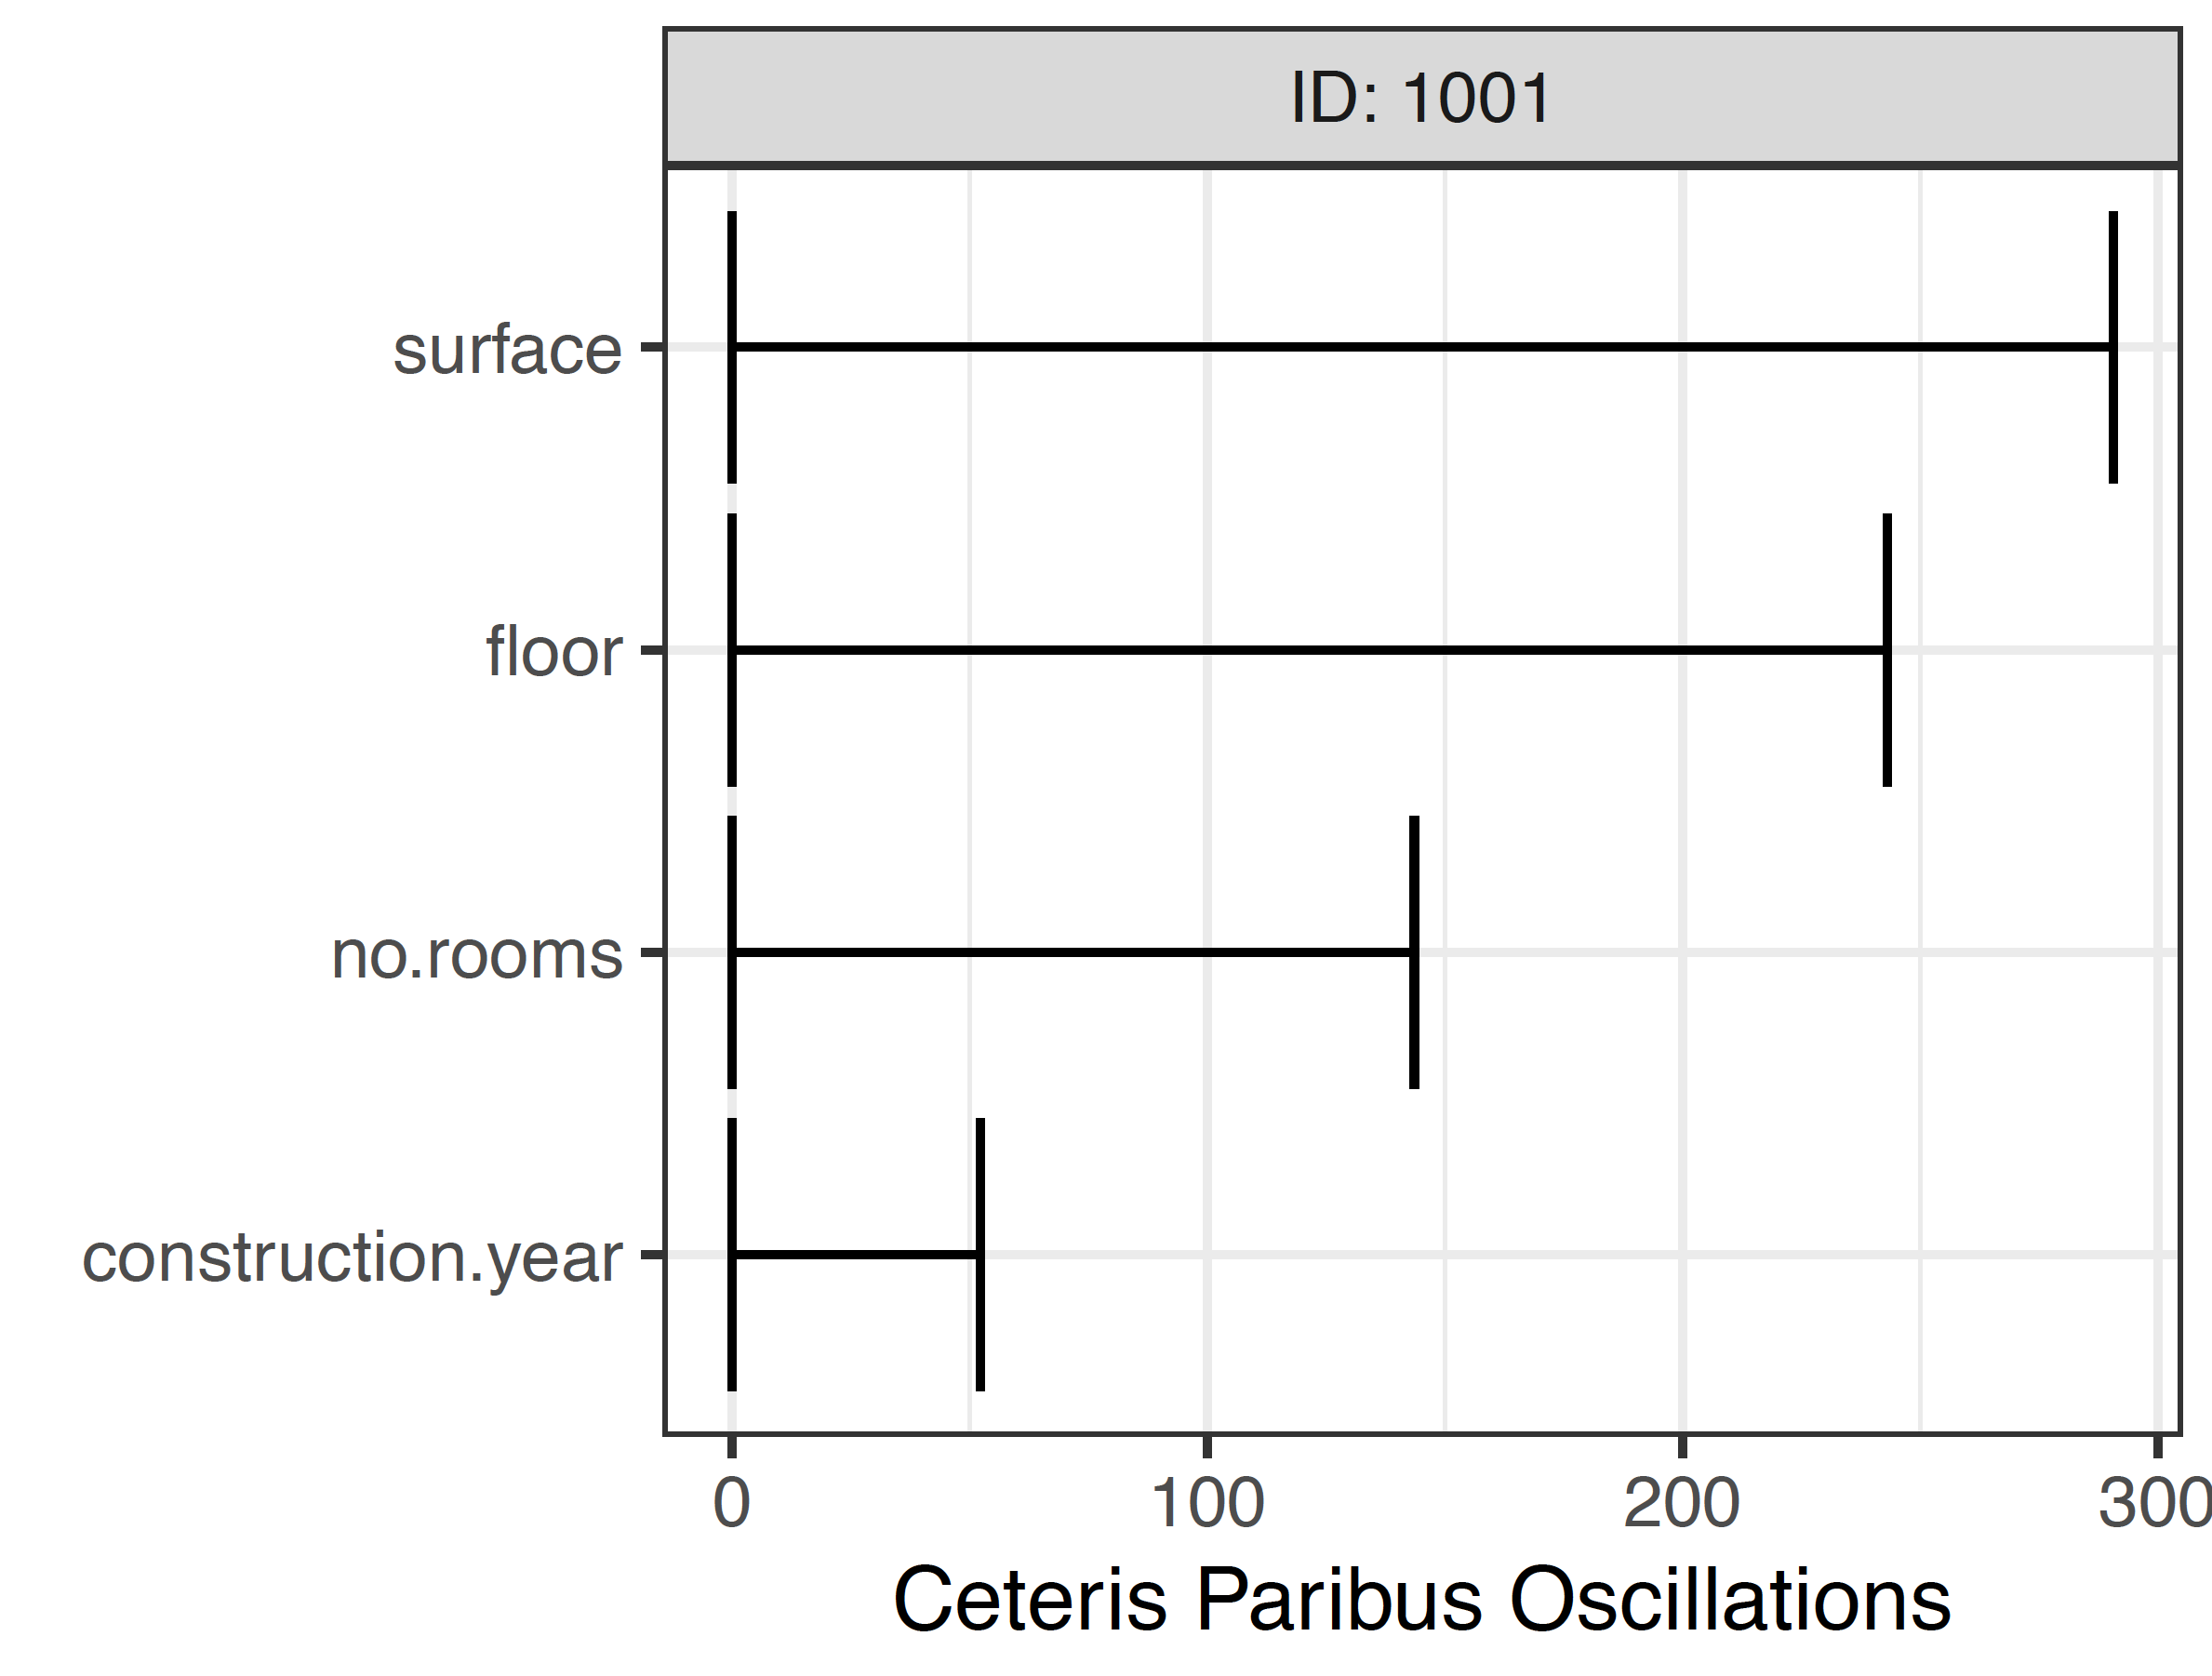
\includegraphics[width=0.4\linewidth]{figure/cp_vip_1} 

}

\caption{(fig:CPVIP1) Variable importance plots calculated for Ceteris Paribus profiles for observation ID: 1001}\label{fig:CPVIP1}
\end{figure}

\textbf{NOTE}

Variable importance for single prediction may be very different than
variable importance for the full model.

For example, consider a model \[
f(x_1, x_2) = x_1 * x_2
\] where variables \(x_1\) and \(x_2\) takes values in \([0,1]\).

From the global perspective both variables are equally important.

But local variable importance is very different. Around point
\(x = (0, 1)\) the importance of \(x_1\) is much larger than \(x_2\).
This is because profile for \(f(z, 1)\) have larger oscillations than
\(f(0, z)\).

\hypertarget{d-profiles}{%
\section{2D profiles}\label{d-profiles}}

The definition of ceteris paribus profiles given in section
\ref{ceterisParibus1d} may be easily extended to two and more variables.
Also definition of CP oscillations \ref{oscillations} have straight
forward generalization for larger number of dimensions. Such
generalisations are usefull when model is non additive. Presence of
pairwise interactions may be detected with 2D Ceteris Paribus plots.

Let's define two-dimensional Ceteris Paribus Profile for model \(f\),
variables \(j\) and \(k\) and point \(x\) as

\[
CP^{f, (j,k), x}(z_1, z_2) := f(x|^{(j,k)} = (z_1,z_2)).
\] I.e. CP profile is a model response obtained for observations created
based on \(x\) with \(j\) and \(k\) coordinates changed to
\((z_1, z_2)\) and all other coordinates kept unchanged.

A natural way to visualise 2D CP profiles is to use a level plot as in
Figure \ref{fig:CP2Dsurflor}.

\begin{figure}

{\centering 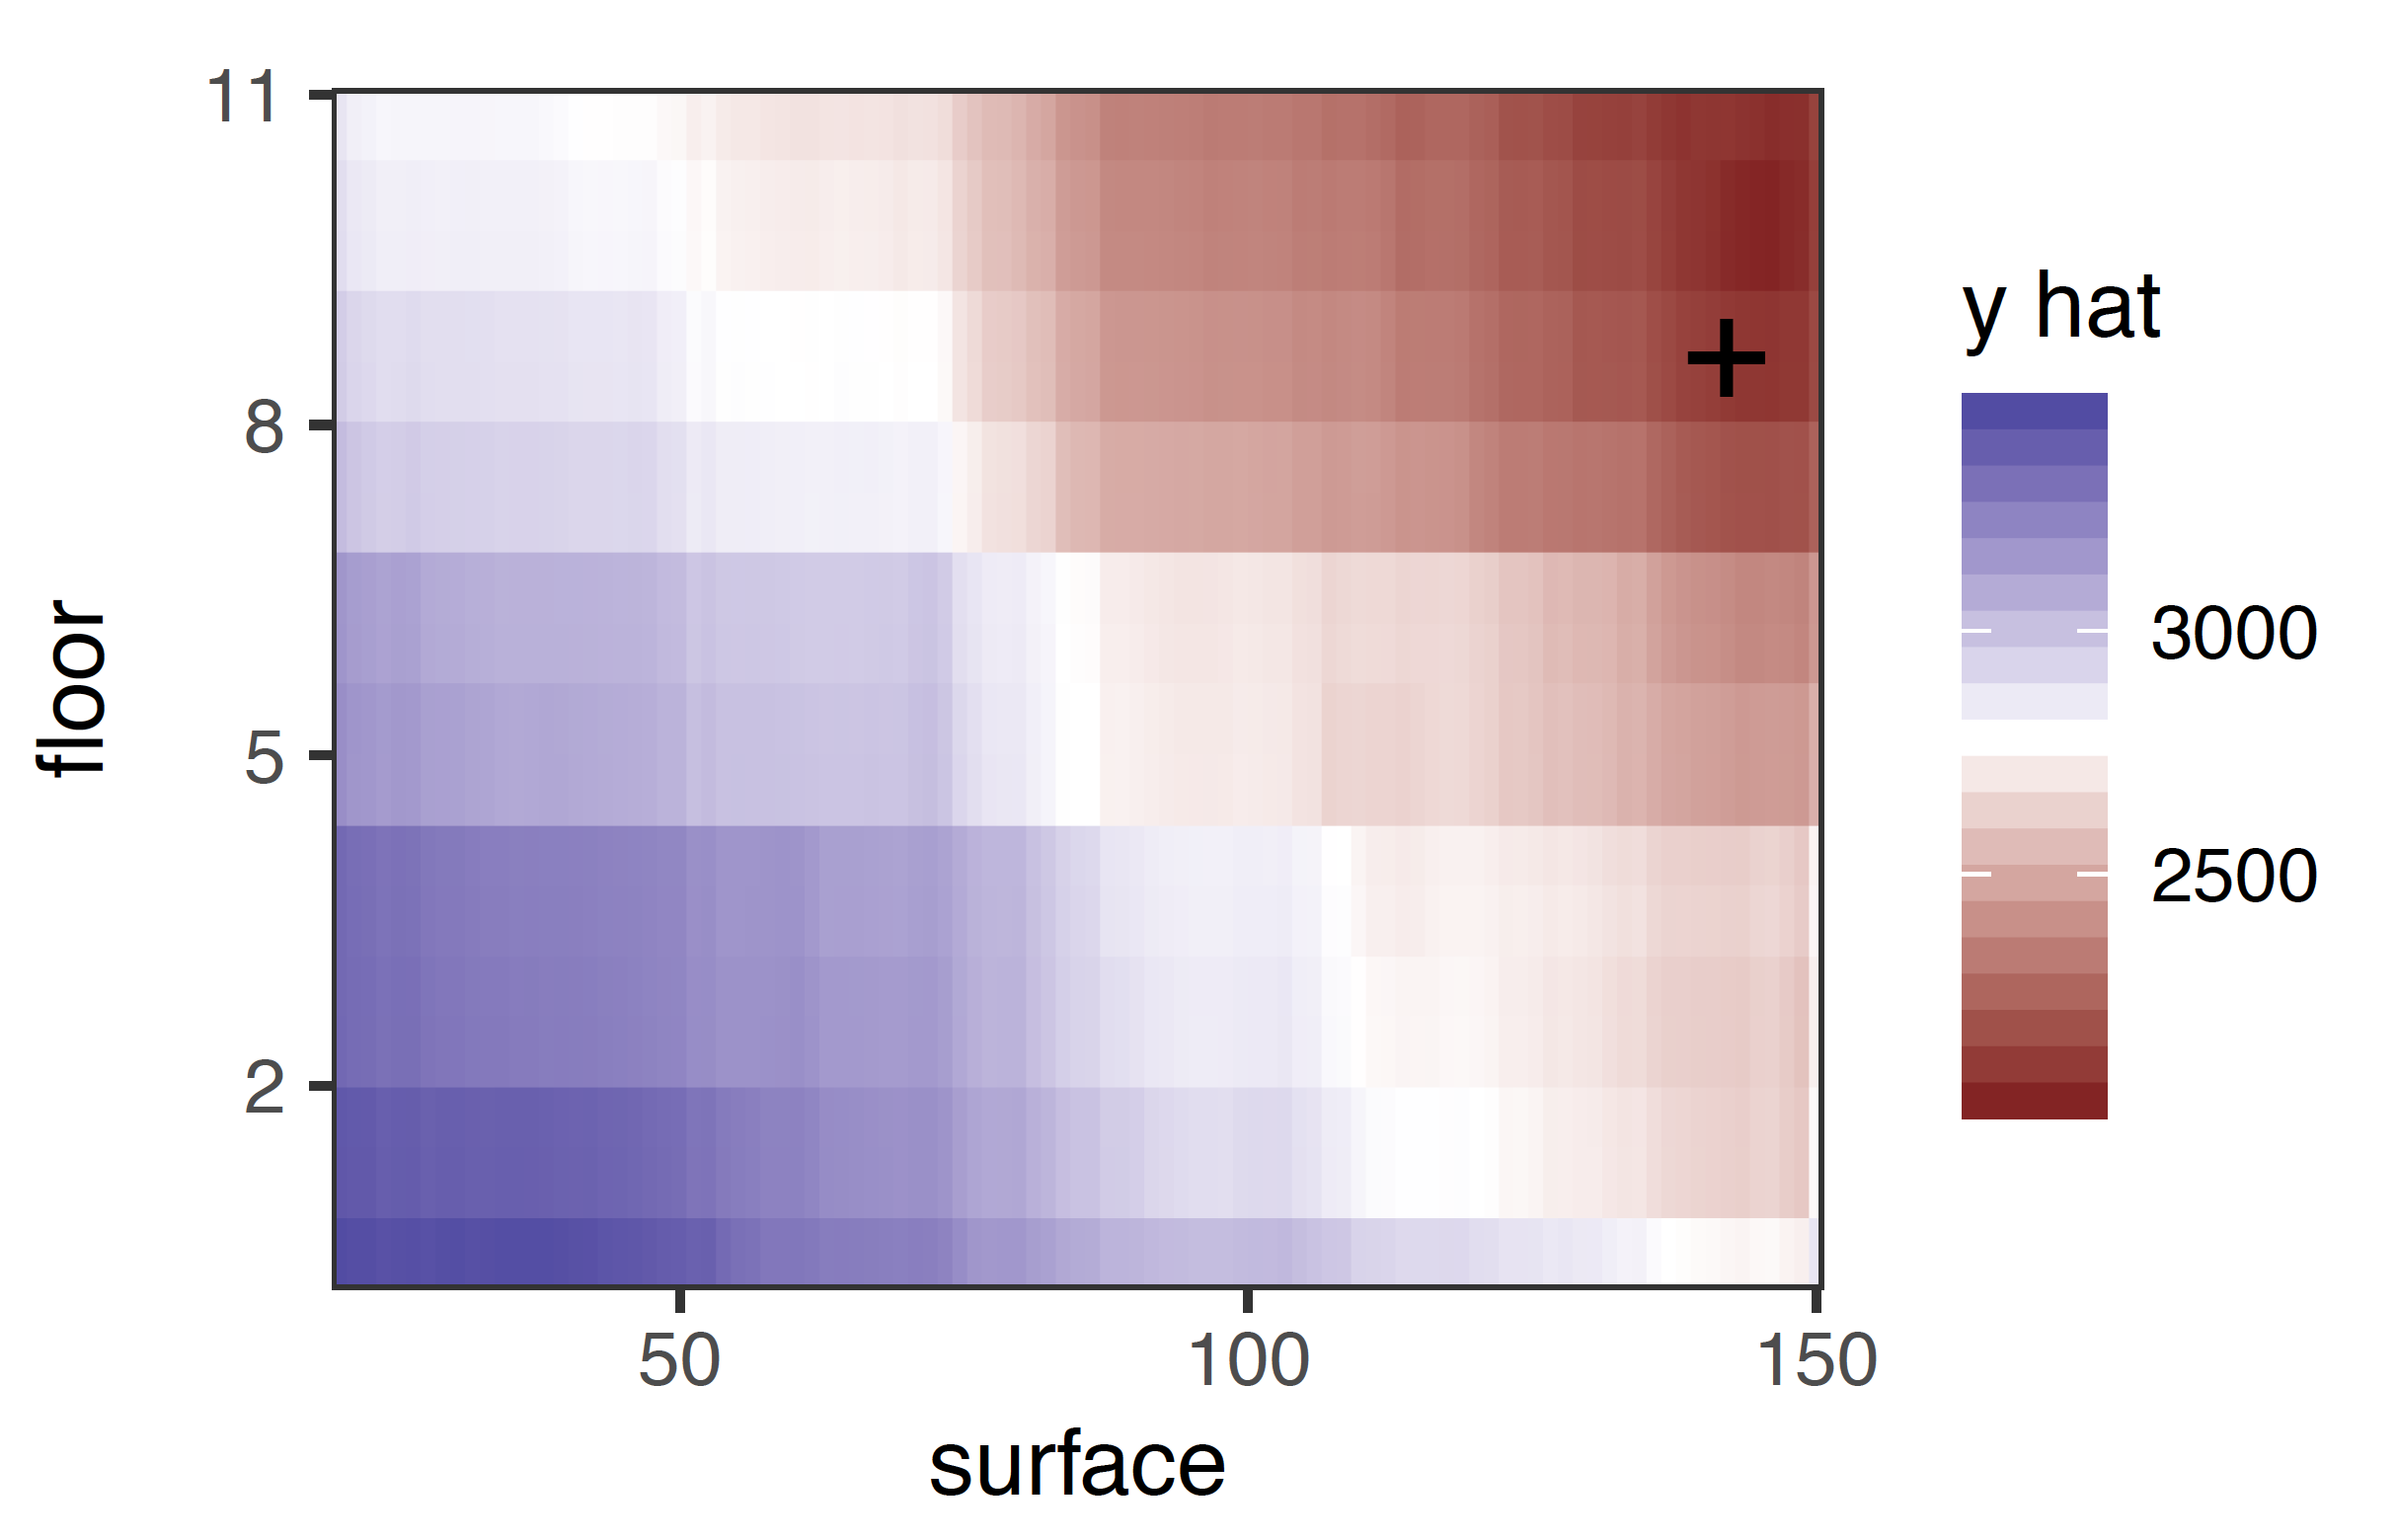
\includegraphics[width=0.6\linewidth]{figure/cp_2d_surf_floor} 

}

\caption{(fig:CP2Dsurflor) Ceteris Paribus plot for a pair of variales. Black cross marks coordinated for the observation of interest. Presented model estimates price of an appartment}\label{fig:CP2Dsurflor}
\end{figure}

If number of variables is small or moderate thein it is possible to
present all pairs of variables. See an example in Figure
\ref{fig:CP2Dall}.

\begin{figure}

{\centering 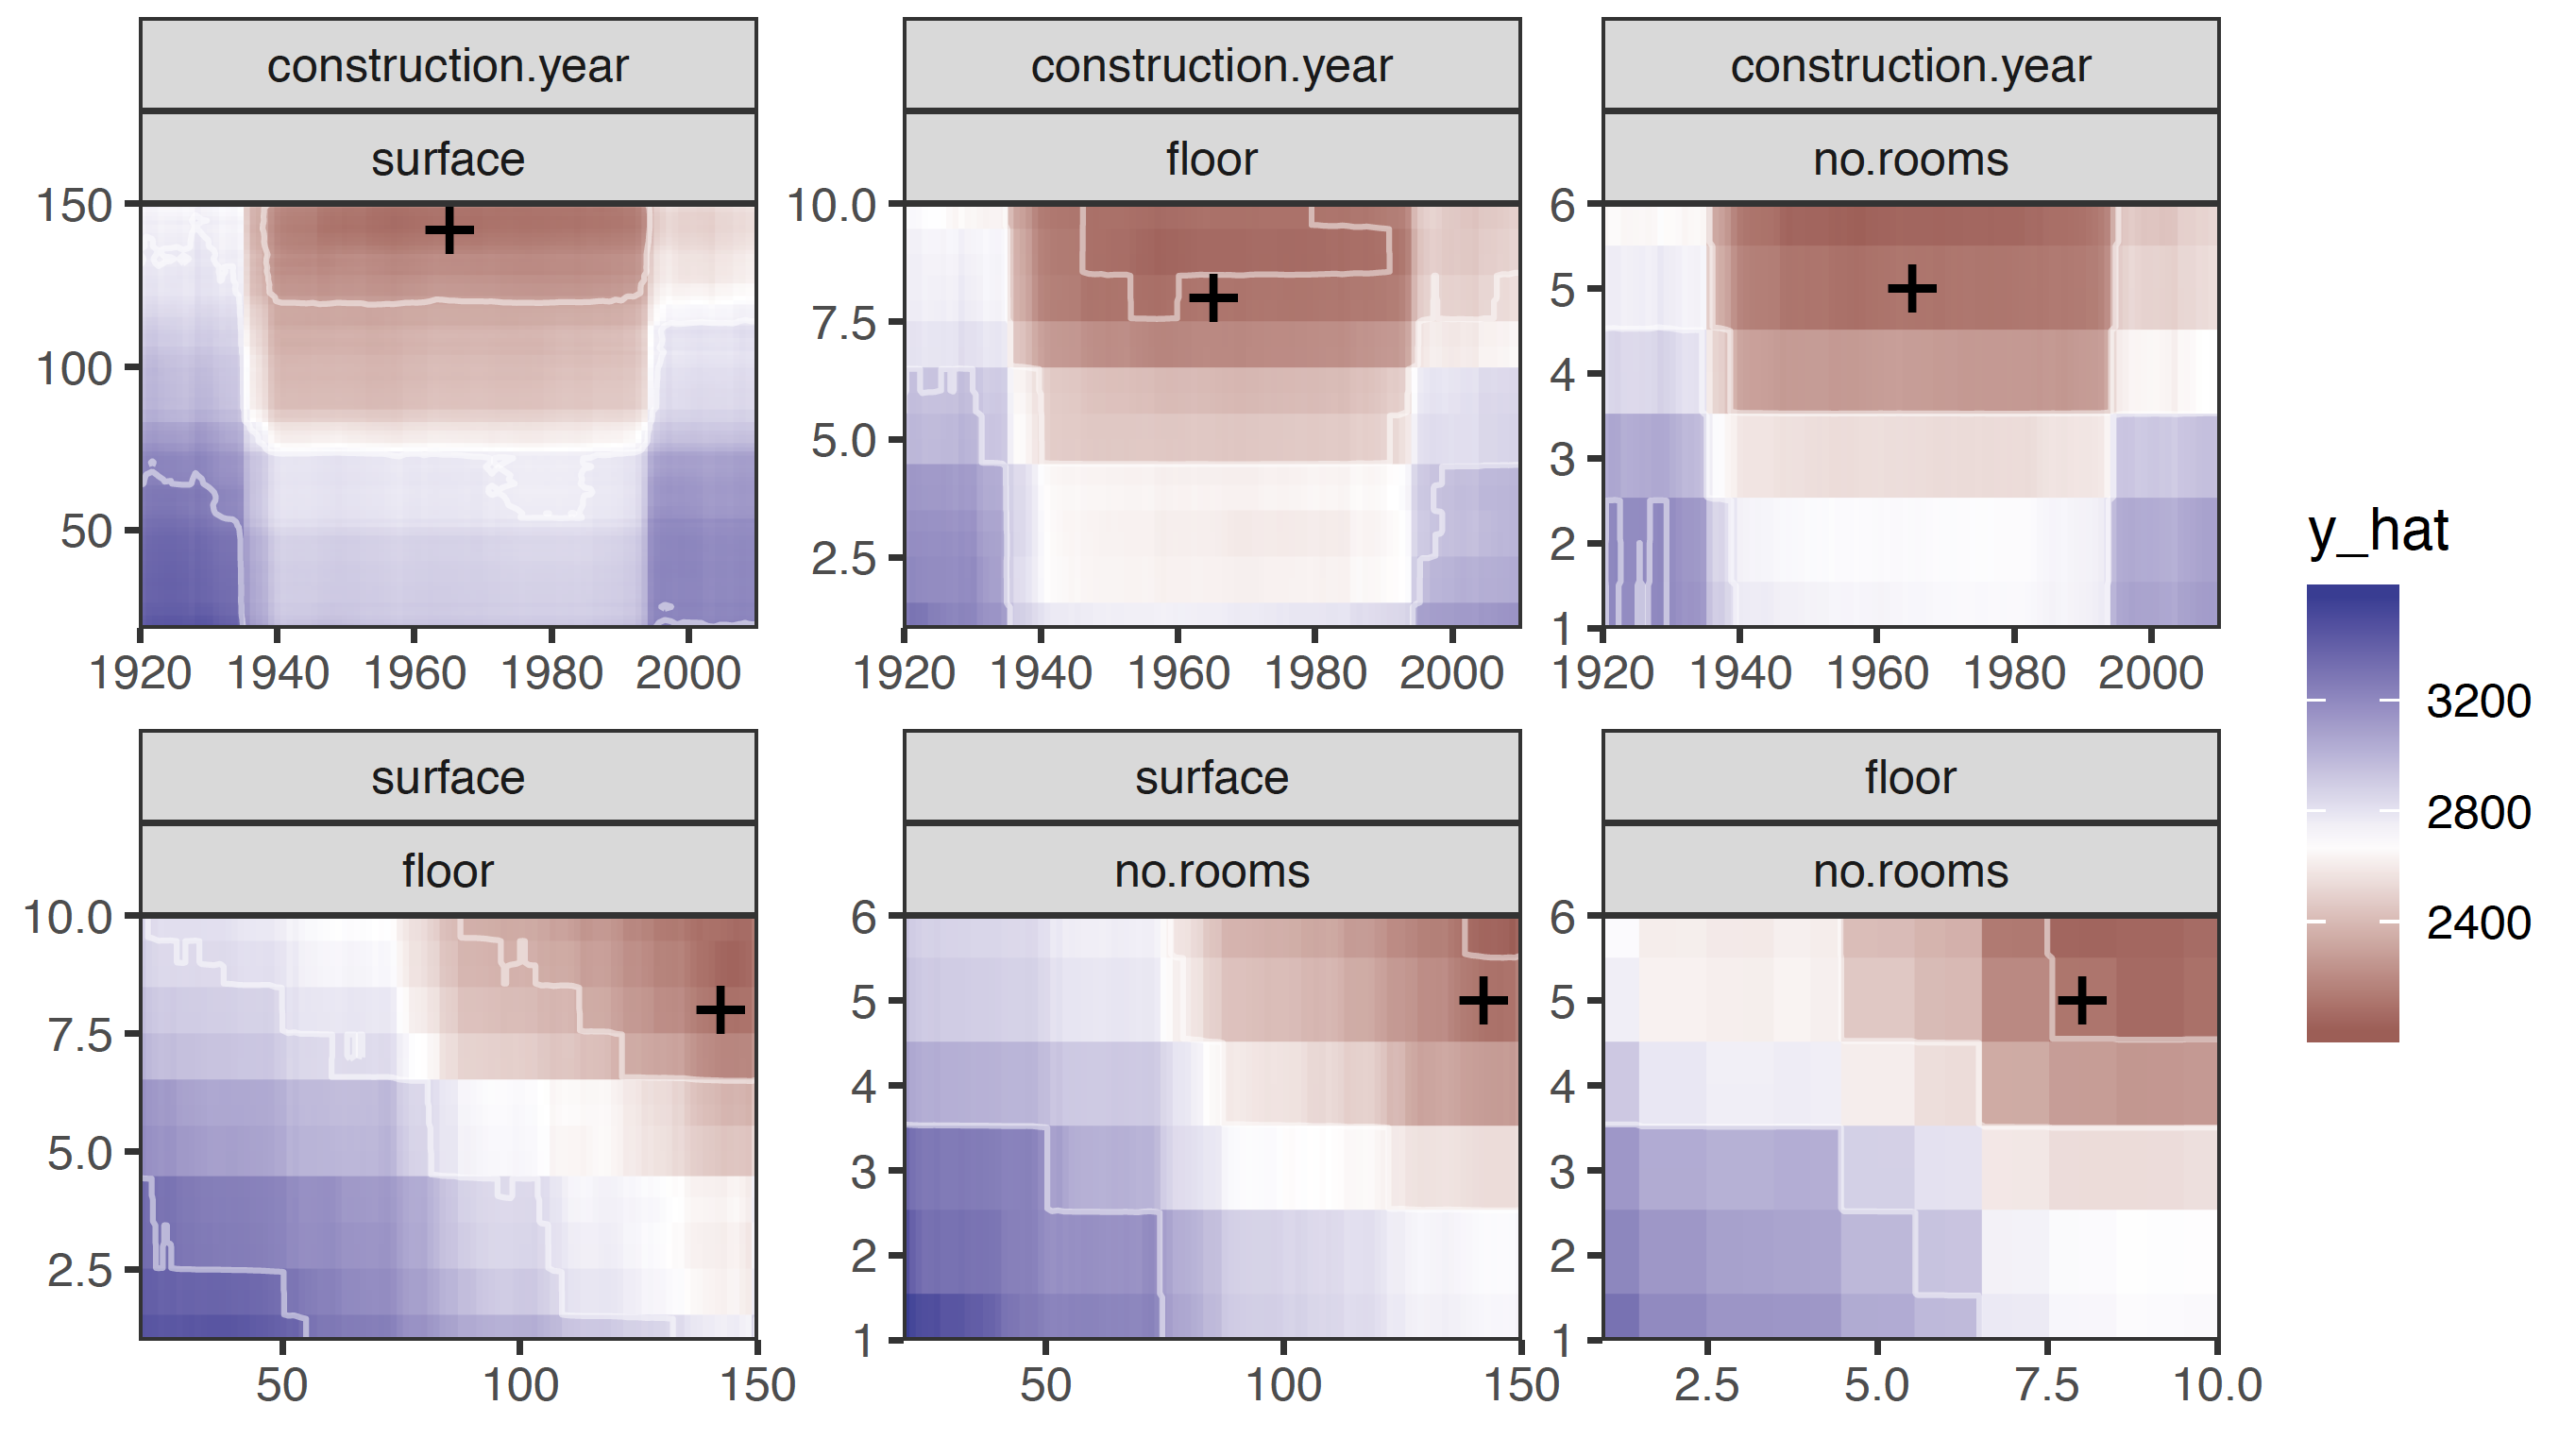
\includegraphics[width=0.9\linewidth]{figure/cp_2d_all} 

}

\caption{(fig:CP2Dall) Ceteris Paribus plot for all pairs of variales.}\label{fig:CP2Dall}
\end{figure}

\hypertarget{local-model-fidelity}{%
\section{Local model fidelity}\label{local-model-fidelity}}

Ceteris Paribus profiles are also a useful tool to validate local model
fidelity. It may happen that global performance of the model is good,
while for some points the local fit is very bad. Local fidelity helps to
understand how good is the model fit around point of interest.

How does it work?

The idea behind fidelity plots is to select some number of points from
the validation dataset that are closes to the point of interest. It's a
similar approach as in k nearest neighbours. Then for these neighbours
we may plot Ceteris Paribus Profiles and check how stable they are.

Also, if we know true taget values for points from the validation
dataset we may plot residuals to show how large are residuals.

An example fidelity plot is presented in Figure \ref{fig:CPfidelity1}.
Black line shows the CP profiles for the point of interest, while grey
lines show CP profiles for neihgbors. Red intervals stand for residuals
and in this example it looks like residuals for neighbours are all
negative. Thus maybe model is biased around the point of interest.

\begin{figure}

{\centering 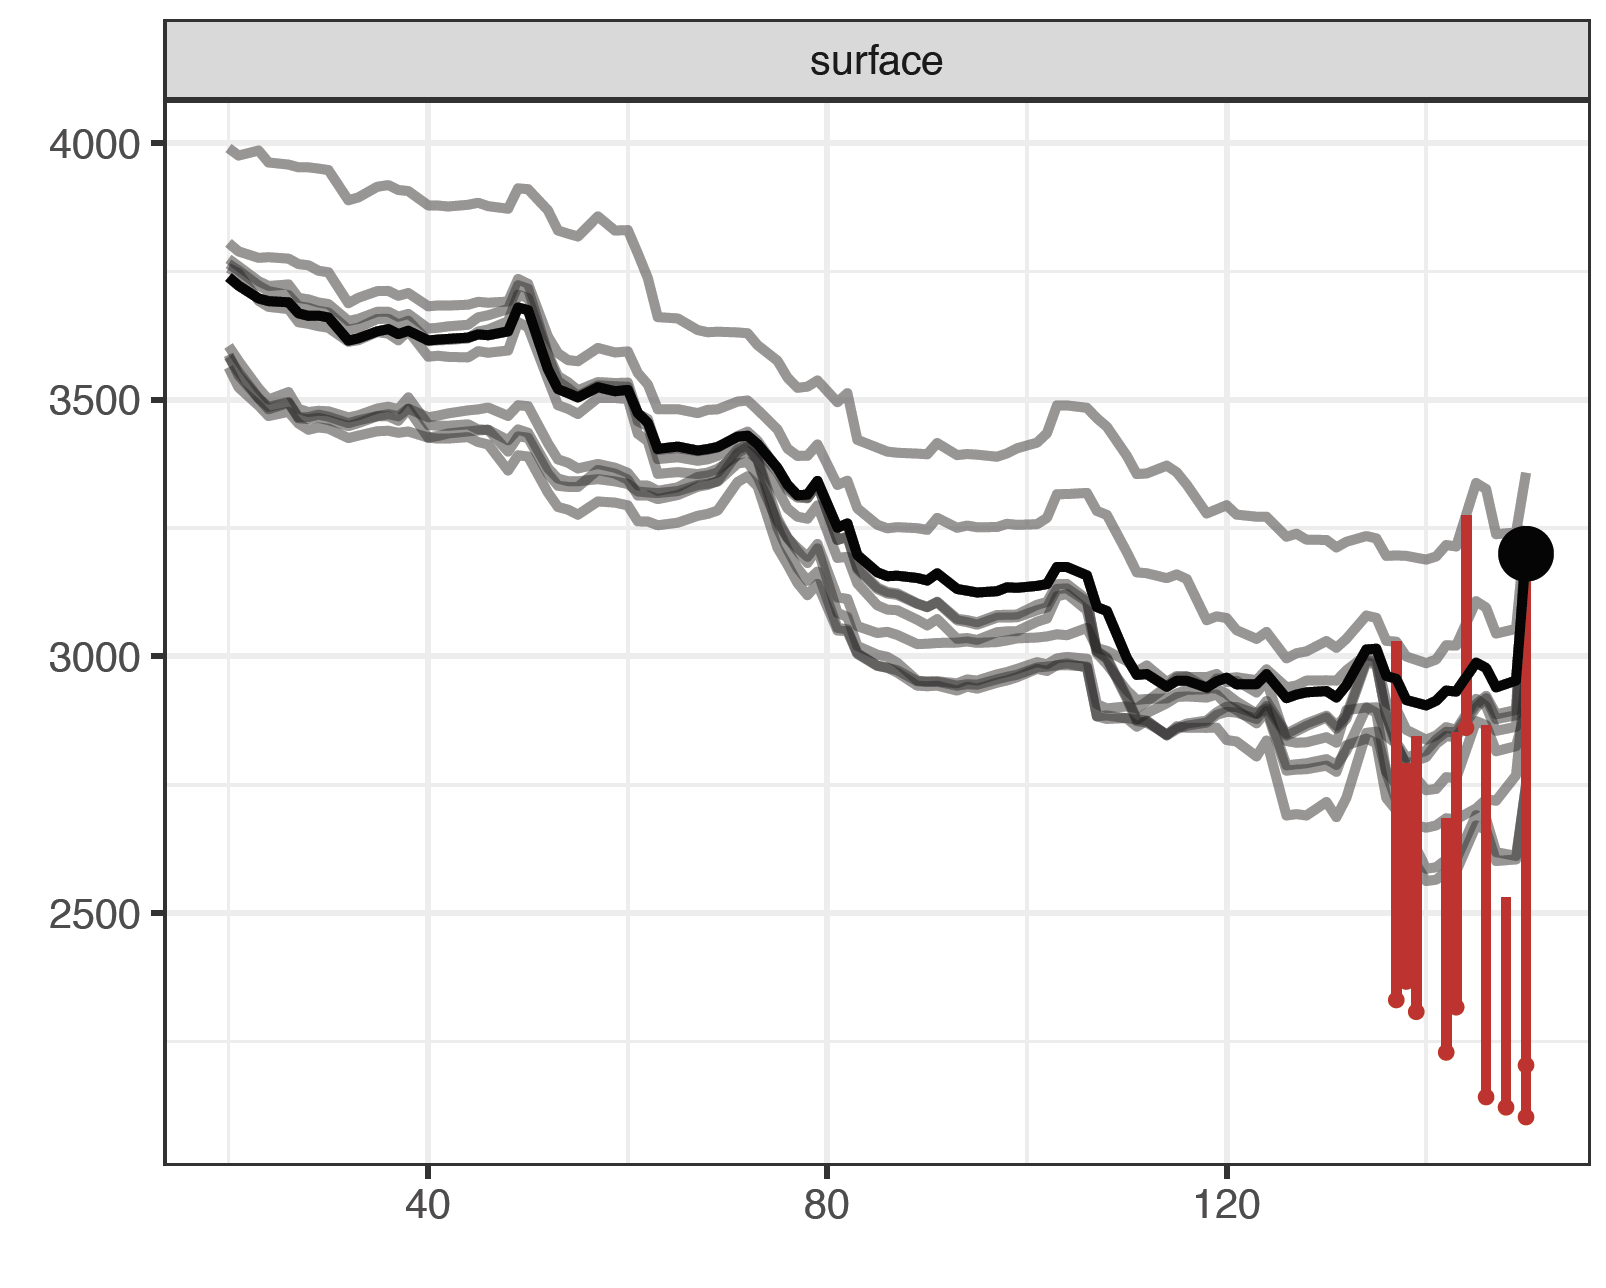
\includegraphics[width=0.7\linewidth]{figure/cp_fidelity_1} 

}

\caption{(fig:CPfidelity1) Local fidelity plots. Black line shows the CP profile for the point of interest. Grey lines show CP profiles for nearest neighbors. Red intervals correspond to residuals. Each red interval starts in a model prediction for a selected neighbor and ends in its true value of target variable.}\label{fig:CPfidelity1}
\end{figure}

This observation may be confirmed by plots that compare distribution of
all residuals against distribution of residuals for neighbors.

See Figure \ref{CPfidelityBoxplot} for an example. Here residuals for
neighbors are shifted towards highest values. This suggests that the
model response is biased around the observation of interest.

\begin{figure}

{\centering 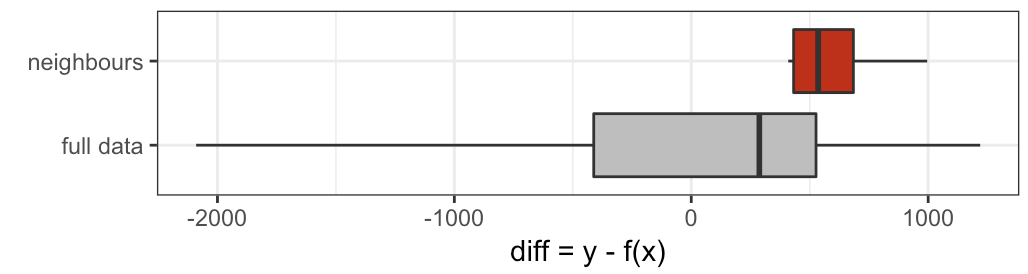
\includegraphics[width=0.7\linewidth]{figure/cp_fidelity_boxplot} 

}

\caption{(fig:CPfidelityBoxplot) Distribution of residuals for whole validation data (grey boxplot) and for selected closes 15 neighbors (red boxplot).}\label{fig:CPfidelityBoxplot}
\end{figure}

\hypertarget{pros-and-cons-1}{%
\section{Pros and cons}\label{pros-and-cons-1}}

Ceteris Paribus principle gives a uniform and extendable approach to
model exploration. Below we summarize key strengths and weaknesses of
this approach.

\textbf{Pros}

\begin{itemize}
\tightlist
\item
  Graphical representation of Ceteris Paribus profile is easy to
  understand.
\item
  Ceteris Paribus profiles are compact and it is easy to fit many models
  or many variables in a small space.
\item
  Ceteris Paribus profiles helps to understand how model response would
  change and how stable it is
\item
  Oscillations calculated for CP profiles helps to select the most
  important variables.
\item
  2D Ceteris Paribus profiles help to identify pairwise interactions
  between variables.
\end{itemize}

\textbf{Cons}

\begin{itemize}
\tightlist
\item
  If variables are correlated (like surface and number of rooms) then
  the `\emph{everything else kept unchanged}' approach leads to
  unrealistic settings.
\item
  Interactions between variables are not visible in 1D plots.
\item
  This tool is not suited for very wide data, like hundreds or thousands
  of variables.
\item
  Visualization of categorical variables is non trivial.
\end{itemize}

\hypertarget{code-snippets-for-r-1}{%
\section{Code snippets for R}\label{code-snippets-for-r-1}}

In this section we present key features of the \texttt{ceterisParibus}
package for R \citep{R-ceterisParibus}. This package covers all features
presented in this chapter. It is available on CRAN and GitHub. Find more
examples at the website of this package
\texttt{https://pbiecek.github.io/ceterisParibus/}.

\textbf{Model preparation}

In this section we will present examples based on the
\texttt{apartments} dataset. See section TODO for more details.

\begin{Shaded}
\begin{Highlighting}[]
\KeywordTok{library}\NormalTok{(}\StringTok{"DALEX"}\NormalTok{)}
\KeywordTok{head}\NormalTok{(apartments)}
\end{Highlighting}
\end{Shaded}

\begin{verbatim}
##   m2.price construction.year surface floor no.rooms    district
## 1     5897              1953      25     3        1 Srodmiescie
## 2     1818              1992     143     9        5     Bielany
## 3     3643              1937      56     1        2       Praga
## 4     3517              1995      93     7        3      Ochota
## 5     3013              1992     144     6        5     Mokotow
## 6     5795              1926      61     6        2 Srodmiescie
\end{verbatim}

The problem here is to predict average price for square meter for an
apartment. Let's build a random forest model with \texttt{randomForest}
package \citep{R-randomForest}.

\begin{Shaded}
\begin{Highlighting}[]
\KeywordTok{library}\NormalTok{(}\StringTok{"randomForest"}\NormalTok{)}
\NormalTok{rf_model <-}\StringTok{ }\KeywordTok{randomForest}\NormalTok{(m2.price }\OperatorTok{~}\StringTok{ }\NormalTok{construction.year }\OperatorTok{+}\StringTok{ }\NormalTok{surface }\OperatorTok{+}\StringTok{ }\NormalTok{floor }\OperatorTok{+}
\StringTok{      }\NormalTok{no.rooms, }\DataTypeTok{data =}\NormalTok{ apartments)}
\NormalTok{rf_model}
\end{Highlighting}
\end{Shaded}

\begin{verbatim}
## 
## Call:
##  randomForest(formula = m2.price ~ construction.year + surface +      floor + no.rooms, data = apartments) 
##                Type of random forest: regression
##                      Number of trees: 500
## No. of variables tried at each split: 1
## 
##           Mean of squared residuals: 486660.5
##                     % Var explained: 40.74
\end{verbatim}

Model exploration with \texttt{ceterisParibus} package is performed in
four steps.

\textbf{1. Create an explainer - wrapper around model and validation
data.}

Since all other functions work in a model agnostic fashion, first we
need to define a wrapper around the model. Here we are using the
\texttt{explain()} function from \texttt{DALEX} package \citep{R-DALEX}.

\begin{Shaded}
\begin{Highlighting}[]
\KeywordTok{library}\NormalTok{(}\StringTok{"DALEX"}\NormalTok{)}
\NormalTok{explainer_rf <-}\StringTok{ }\KeywordTok{explain}\NormalTok{(rf_model,}
      \DataTypeTok{data =}\NormalTok{ apartmentsTest, }\DataTypeTok{y =}\NormalTok{ apartmentsTest}\OperatorTok{$}\NormalTok{m2.price)}
\NormalTok{explainer_rf}
\end{Highlighting}
\end{Shaded}

\begin{verbatim}
## Model label:  randomForest 
## Model class:  randomForest.formula,randomForest 
## Data head  :
##      m2.price construction.year surface floor no.rooms    district
## 1001     4644              1976     131     3        5 Srodmiescie
## 1002     3082              1978     112     9        4     Mokotow
\end{verbatim}

\textbf{2. Define point of interest.}

Certeris Paribus profiles explore model around a single point.

\begin{Shaded}
\begin{Highlighting}[]
\NormalTok{new_apartment <-}\StringTok{ }\KeywordTok{data.frame}\NormalTok{(}\DataTypeTok{construction.year =} \DecValTok{1965}\NormalTok{, }\DataTypeTok{no.rooms =} \DecValTok{5}\NormalTok{, }\DataTypeTok{surface =} \DecValTok{142}\NormalTok{, }\DataTypeTok{floor =} \DecValTok{8}\NormalTok{)}
\NormalTok{new_apartment}
\end{Highlighting}
\end{Shaded}

\begin{verbatim}
##   construction.year no.rooms surface floor
## 1              1965        5     142     8
\end{verbatim}

\begin{Shaded}
\begin{Highlighting}[]
\KeywordTok{predict}\NormalTok{(rf_model, new_apartment)}
\end{Highlighting}
\end{Shaded}

\begin{verbatim}
##        1 
## 2311.108
\end{verbatim}

\textbf{3. Calculate CP profiles}

The \texttt{ceteris\_paribus()} function calculates CP profiles for
selected model around selected observation.

By default CP profiles are calculated for all numerical variables. Use
the \texttt{variables} argument to select subset of interesting
variables. The result from \texttt{ceteris\_paribus()}function is a data
frame with model predictions for modified points around the point of
interest.

\begin{Shaded}
\begin{Highlighting}[]
\KeywordTok{library}\NormalTok{(}\StringTok{"ceterisParibus"}\NormalTok{)}
\NormalTok{cp_rf <-}\StringTok{ }\KeywordTok{ceteris_paribus}\NormalTok{(explainer_rf, new_apartment, }
                            \DataTypeTok{variables =} \KeywordTok{c}\NormalTok{(}\StringTok{"construction.year"}\NormalTok{, }\StringTok{"floor"}\NormalTok{))}
\NormalTok{cp_rf}
\end{Highlighting}
\end{Shaded}

\begin{verbatim}
## Top profiles    : 
##     construction.year no.rooms surface floor   _yhat_           _vname_
## 1                1920        5     142     8 3091.884 construction.year
## 1.1              1921        5     142     8 3116.261 construction.year
## 1.2              1922        5     142     8 3110.009 construction.year
## 1.3              1923        5     142     8 3071.335 construction.year
## 1.4              1923        5     142     8 3071.335 construction.year
## 1.5              1924        5     142     8 3063.594 construction.year
##     _ids_      _label_
## 1       1 randomForest
## 1.1     1 randomForest
## 1.2     1 randomForest
## 1.3     1 randomForest
## 1.4     1 randomForest
## 1.5     1 randomForest
## 
## 
## Top observations:
##   construction.year no.rooms surface floor   _yhat_      _label_
## 1              1965        5     142     8 2311.108 randomForest
\end{verbatim}

\textbf{4. Plot CP profiles.}

Generic \texttt{plot()} function plot CP profiles. It returns a
\texttt{ggplot2} object that can be polished if needed. Use additional
arguments of this function to select colors and sizes for elements
visible in the plot.

\begin{Shaded}
\begin{Highlighting}[]
\KeywordTok{plot}\NormalTok{(cp_rf) }
\end{Highlighting}
\end{Shaded}

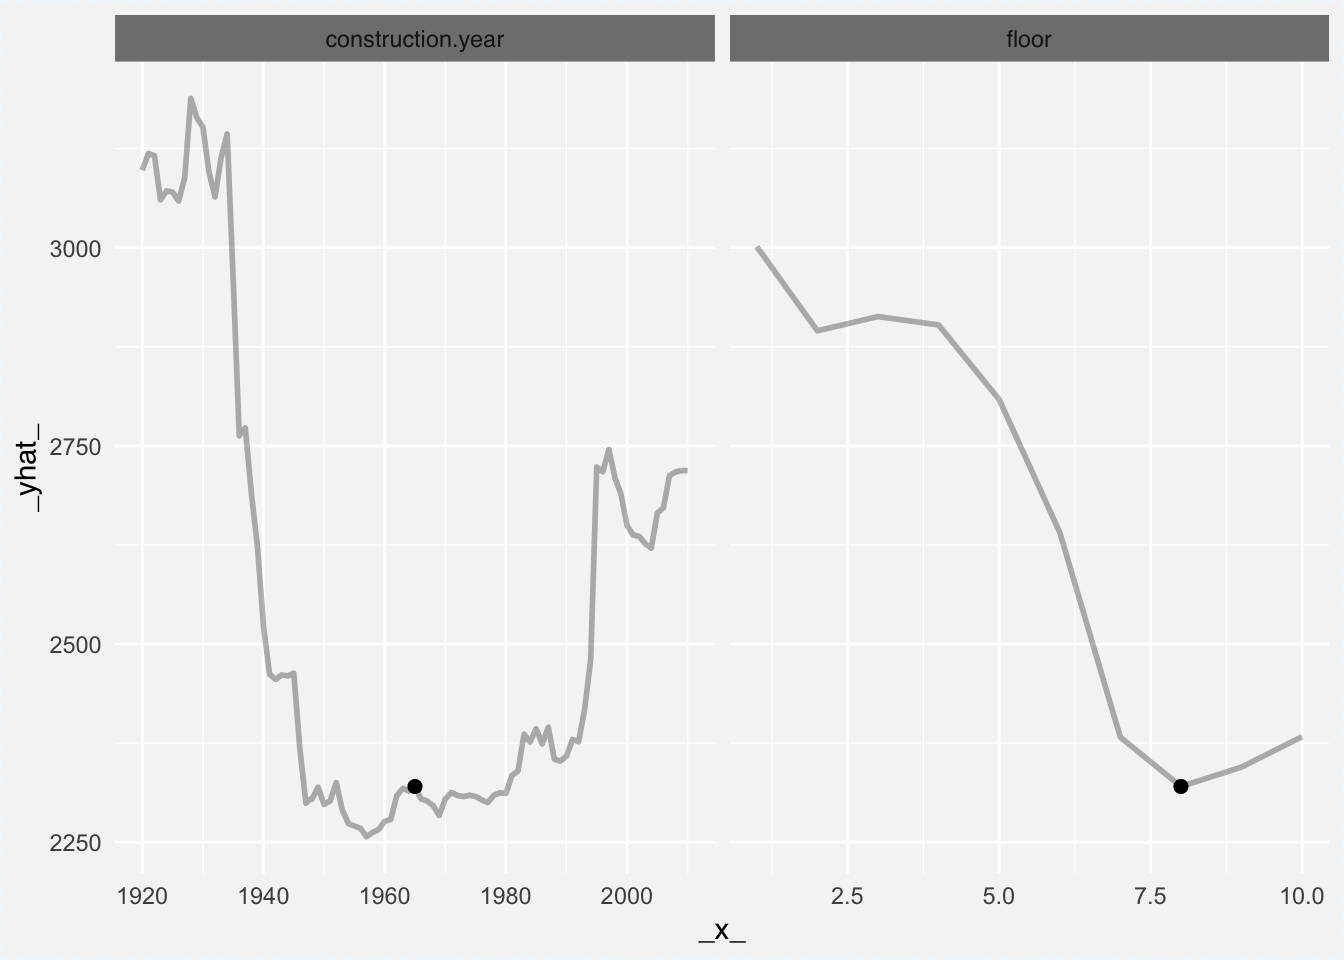
\includegraphics{PM_VEE_files/figure-latex/unnamed-chunk-15-1.pdf}

One of very useful features of \texttt{ceterisParibus} explainers is
that profiles for two or more models may be superimposed in a single
plot. This helps in model comparisons.

Let's create a linear model for this dataset and repeat steps 1-3 for
the lm model.

\begin{Shaded}
\begin{Highlighting}[]
\NormalTok{lm_model <-}\StringTok{ }\KeywordTok{lm}\NormalTok{(m2.price }\OperatorTok{~}\StringTok{ }\NormalTok{construction.year }\OperatorTok{+}\StringTok{ }\NormalTok{surface }\OperatorTok{+}\StringTok{ }\NormalTok{floor }\OperatorTok{+}
\StringTok{      }\NormalTok{no.rooms, }\DataTypeTok{data =}\NormalTok{ apartments)}
\NormalTok{explainer_lm <-}\StringTok{ }\KeywordTok{explain}\NormalTok{(lm_model,}
      \DataTypeTok{data =}\NormalTok{ apartmentsTest, }\DataTypeTok{y =}\NormalTok{ apartmentsTest}\OperatorTok{$}\NormalTok{m2.price)}
\NormalTok{cp_lm <-}\StringTok{ }\KeywordTok{ceteris_paribus}\NormalTok{(explainer_lm, new_apartment, }
                            \DataTypeTok{variables =} \KeywordTok{c}\NormalTok{(}\StringTok{"construction.year"}\NormalTok{, }\StringTok{"floor"}\NormalTok{))}
\end{Highlighting}
\end{Shaded}

Now we can use function \texttt{plot()} to compare both models in a
single chart. Additional argument \texttt{color\ =\ "\_label\_"} set
color as a key for model.

\begin{Shaded}
\begin{Highlighting}[]
\KeywordTok{plot}\NormalTok{(cp_rf, cp_lm, }\DataTypeTok{color =} \StringTok{"_label_"}\NormalTok{)}
\end{Highlighting}
\end{Shaded}

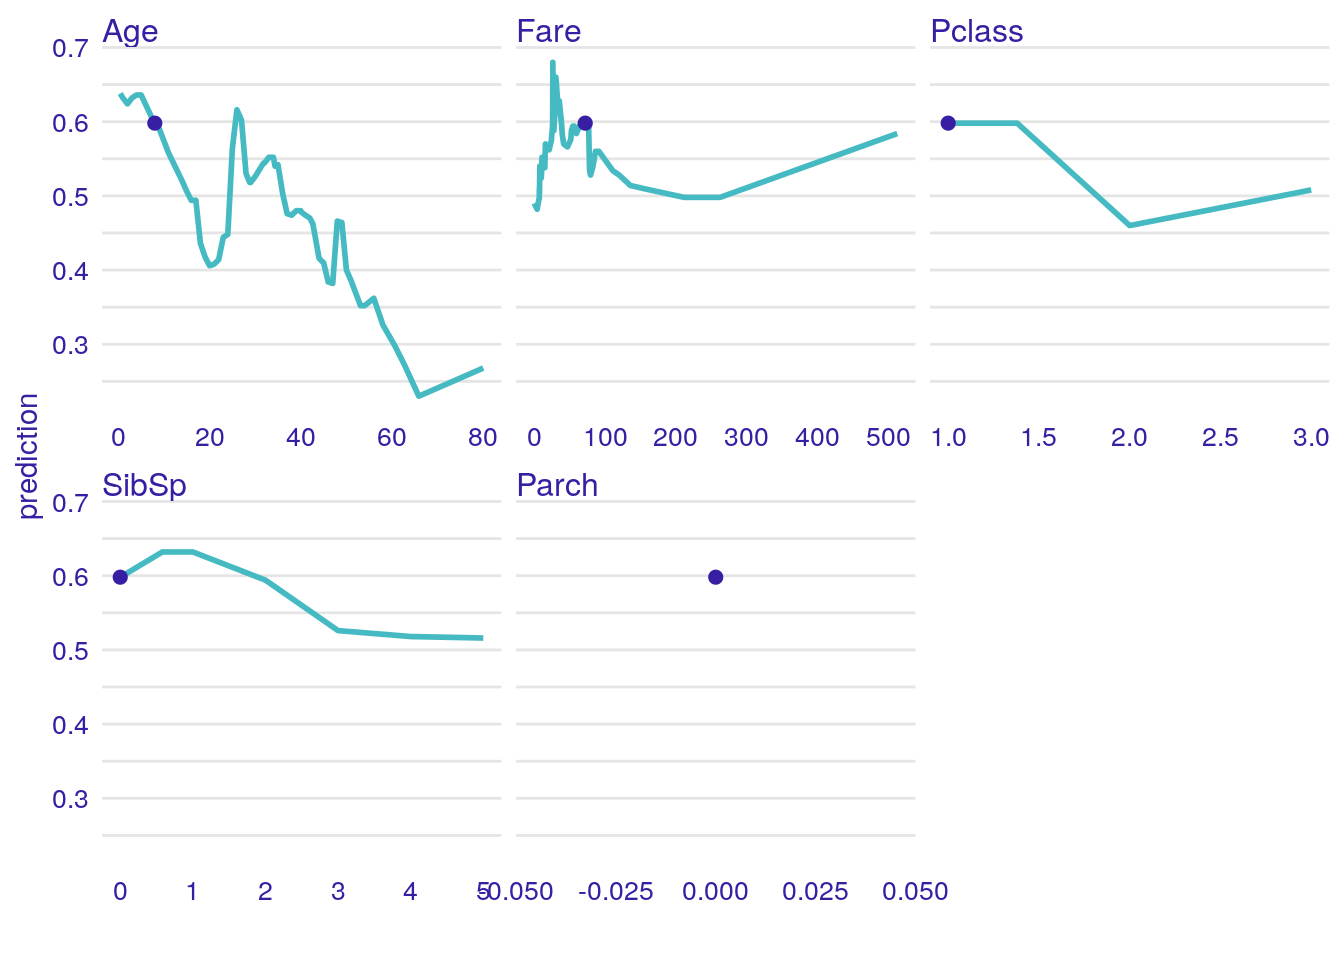
\includegraphics{PM_VEE_files/figure-latex/unnamed-chunk-17-1.pdf}

\textbf{Oscillations}

The \texttt{calculate\_oscillations()} function calculates oscillations
for CP profiles.

\begin{Shaded}
\begin{Highlighting}[]
\NormalTok{cp_rf_all <-}\StringTok{ }\KeywordTok{ceteris_paribus}\NormalTok{(explainer_rf, new_apartment)}
\NormalTok{co_rf_all <-}\StringTok{ }\KeywordTok{calculate_oscillations}\NormalTok{(cp_rf_all)}
\NormalTok{co_rf_all}
\end{Highlighting}
\end{Shaded}

\begin{verbatim}
##             _vname_ _ids_ oscillations
## 2           surface     1     632.5026
## 4          no.rooms     1     439.1318
## 3             floor     1     343.6137
## 1 construction.year     1     243.3204
\end{verbatim}

\begin{Shaded}
\begin{Highlighting}[]
\KeywordTok{plot}\NormalTok{(co_rf_all)}
\end{Highlighting}
\end{Shaded}

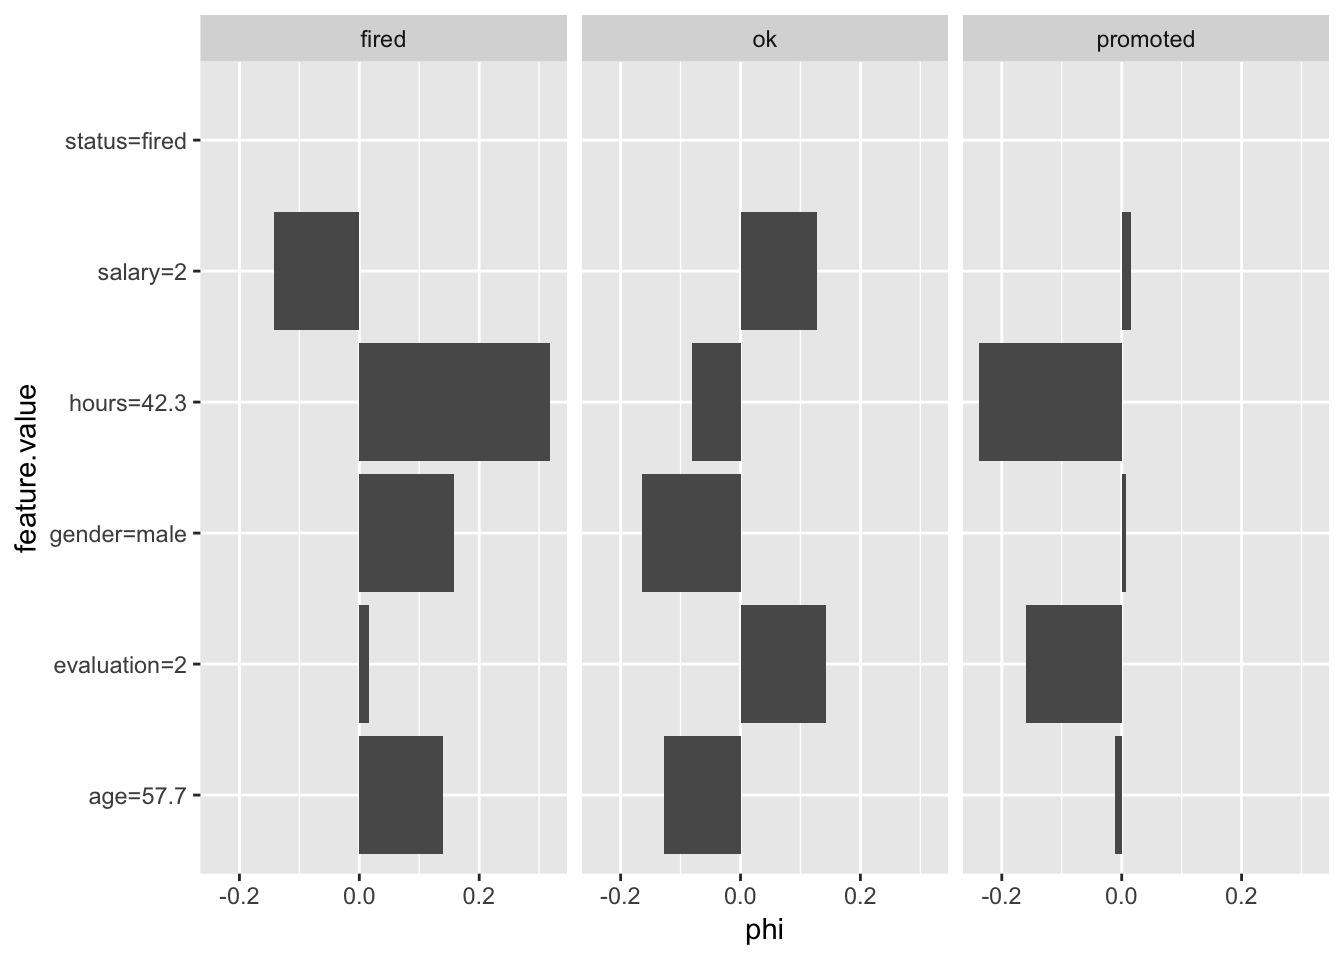
\includegraphics{PM_VEE_files/figure-latex/unnamed-chunk-18-1.pdf}

\textbf{2D Ceteris Paribus profiles}

And the \texttt{what\_if\_2d()} function calculates 2D CP profiles.

\begin{Shaded}
\begin{Highlighting}[]
\NormalTok{wi_rf_2d <-}\StringTok{ }\KeywordTok{what_if_2d}\NormalTok{(explainer_rf, }\DataTypeTok{observation =}\NormalTok{ new_apartment, }
                 \DataTypeTok{selected_variables =} \KeywordTok{c}\NormalTok{(}\StringTok{"surface"}\NormalTok{,}\StringTok{"floor"}\NormalTok{, }\StringTok{"construction.year"}\NormalTok{))}
\KeywordTok{plot}\NormalTok{(wi_rf_2d, }\DataTypeTok{split_ncol =} \DecValTok{2}\NormalTok{)}
\end{Highlighting}
\end{Shaded}

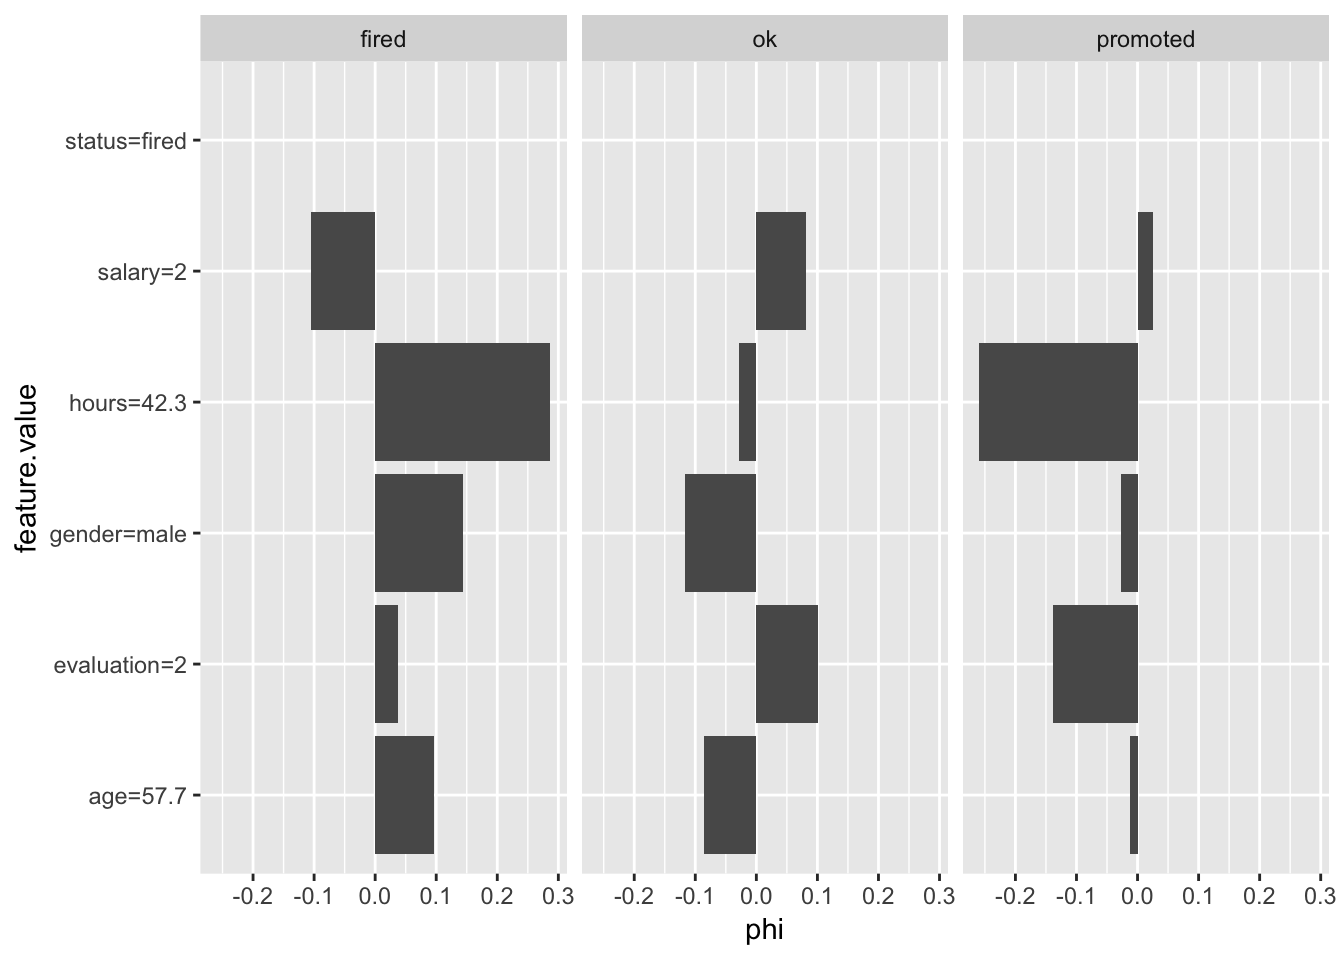
\includegraphics{PM_VEE_files/figure-latex/unnamed-chunk-19-1.pdf}

\hypertarget{model-level-explanations}{%
\chapter*{Model level explanations}\label{model-level-explanations}}
\addcontentsline{toc}{chapter}{Model level explanations}

\hypertarget{introduction-3}{%
\chapter{Introduction}\label{introduction-3}}

\hypertarget{example-price-prediction}{%
\section{Example: Price prediction}\label{example-price-prediction}}

\citep{R-DALEX}

In this chapter we show examples for three predictive models trained on
\texttt{apartments} dataset from the \texttt{DALEX} package. Random
Forest model (elastic but biased), Support Vector Machines model (large
variance on boundaries) and Linear Model (stable but not very elastic).
Presented examples are for regression (prediction of square meter
price), but the CP profiles may be used in the same way for
classification.

\begin{Shaded}
\begin{Highlighting}[]
\KeywordTok{library}\NormalTok{(}\StringTok{"DALEX"}\NormalTok{)}
\CommentTok{# Linear model trained on apartments data}
\NormalTok{model_lm <-}\StringTok{ }\KeywordTok{lm}\NormalTok{(m2.price }\OperatorTok{~}\StringTok{ }\NormalTok{construction.year }\OperatorTok{+}\StringTok{ }\NormalTok{surface }\OperatorTok{+}\StringTok{ }\NormalTok{floor }\OperatorTok{+}\StringTok{ }
\StringTok{                      }\NormalTok{no.rooms }\OperatorTok{+}\StringTok{ }\NormalTok{district, }\DataTypeTok{data =}\NormalTok{ apartments)}

\KeywordTok{library}\NormalTok{(}\StringTok{"randomForest"}\NormalTok{)}
\KeywordTok{set.seed}\NormalTok{(}\DecValTok{59}\NormalTok{)}
\CommentTok{# Random Forest model trained on apartments data}
\NormalTok{model_rf <-}\StringTok{ }\KeywordTok{randomForest}\NormalTok{(m2.price }\OperatorTok{~}\StringTok{ }\NormalTok{construction.year }\OperatorTok{+}\StringTok{ }\NormalTok{surface }\OperatorTok{+}\StringTok{ }\NormalTok{floor }\OperatorTok{+}\StringTok{ }
\StringTok{                      }\NormalTok{no.rooms }\OperatorTok{+}\StringTok{ }\NormalTok{district, }\DataTypeTok{data =}\NormalTok{ apartments)}

\KeywordTok{library}\NormalTok{(}\StringTok{"e1071"}\NormalTok{)}
\CommentTok{# Support Vector Machinesr model trained on apartments data}
\NormalTok{model_svm <-}\StringTok{ }\KeywordTok{svm}\NormalTok{(m2.price }\OperatorTok{~}\StringTok{ }\NormalTok{construction.year }\OperatorTok{+}\StringTok{ }\NormalTok{surface }\OperatorTok{+}\StringTok{ }\NormalTok{floor }\OperatorTok{+}\StringTok{ }
\StringTok{                         }\NormalTok{no.rooms }\OperatorTok{+}\StringTok{ }\NormalTok{district, }\DataTypeTok{data =}\NormalTok{ apartments)}
\end{Highlighting}
\end{Shaded}

For these models we use \texttt{DALEX} explainers created with
\texttt{explain()} function. There exapliners wrap models, predict
functions and validation data.

\begin{Shaded}
\begin{Highlighting}[]
\NormalTok{explainer_lm <-}\StringTok{ }\KeywordTok{explain}\NormalTok{(model_lm, }
                       \DataTypeTok{data =}\NormalTok{ apartmentsTest[,}\DecValTok{2}\OperatorTok{:}\DecValTok{6}\NormalTok{], }\DataTypeTok{y =}\NormalTok{ apartmentsTest}\OperatorTok{$}\NormalTok{m2.price)}
\NormalTok{explainer_rf <-}\StringTok{ }\KeywordTok{explain}\NormalTok{(model_rf, }
                       \DataTypeTok{data =}\NormalTok{ apartmentsTest[,}\DecValTok{2}\OperatorTok{:}\DecValTok{6}\NormalTok{], }\DataTypeTok{y =}\NormalTok{ apartmentsTest}\OperatorTok{$}\NormalTok{m2.price)}
\NormalTok{explainer_svm <-}\StringTok{ }\KeywordTok{explain}\NormalTok{(model_svm, }
                       \DataTypeTok{data =}\NormalTok{ apartmentsTest[,}\DecValTok{2}\OperatorTok{:}\DecValTok{6}\NormalTok{], }\DataTypeTok{y =}\NormalTok{ apartmentsTest}\OperatorTok{$}\NormalTok{m2.price)}
\end{Highlighting}
\end{Shaded}

Examples presented in this chapter are generated with the
\texttt{ceterisParibus} package in version 0.3.1.

\begin{Shaded}
\begin{Highlighting}[]
\KeywordTok{library}\NormalTok{(}\StringTok{"ceterisParibus"}\NormalTok{)}
\end{Highlighting}
\end{Shaded}

\hypertarget{variable-importance}{%
\chapter{Variable Importance}\label{variable-importance}}

Feature selection

\hypertarget{marginal-response}{%
\chapter{Marginal Response}\label{marginal-response}}

Feature extraction

\hypertarget{partial-dependency-plots}{%
\section{Partial Dependency Plots}\label{partial-dependency-plots}}

Accumulated Local Effects (ALE) Plots

\citep{R-ALEPlot}

\begin{Shaded}
\begin{Highlighting}[]
\KeywordTok{library}\NormalTok{(ALEPlot)}
\end{Highlighting}
\end{Shaded}

Interactions - extraction

\hypertarget{merging-path-plots}{%
\section{Merging Path Plots}\label{merging-path-plots}}

\citep{R-factorMerger}

\begin{Shaded}
\begin{Highlighting}[]
\KeywordTok{library}\NormalTok{(factorMerger)}
\end{Highlighting}
\end{Shaded}

\hypertarget{performance-diagnostic}{%
\chapter{Performance Diagnostic}\label{performance-diagnostic}}

Model selection

\hypertarget{residual-diagnostic}{%
\chapter{Residual Diagnostic}\label{residual-diagnostic}}

Model validation

\hypertarget{other-topics}{%
\chapter{Other topics}\label{other-topics}}

\bibliography{book.bib,packages.bib}


\end{document}
